\documentclass[oneside,12pt]{wipb}

\usepackage{float}
\usepackage{amsmath}
\usepackage{amsthm}
\usepackage{amssymb} %symbole strza�ek
\usepackage{amsfonts}
\usepackage{latexsym}
\usepackage{fancyhdr} 
\usepackage{array}
\theoremstyle{definition}
\newcommand{\re}{\mathbb{R}}  % definiowanie liczb RZECZYWISTYCH 
\newtheorem{definition}{Definicja}%[section]
\newtheorem{ex}{Przyk�ad}%[section]
\newtheorem{theorem}{Twierdzenie}%[section]
\newtheorem{uw}{Uwaga}
\newtheorem{wniosek}{Wniosek}
\newtheorem*{dowod*}{Dow�d}
\newtheorem{stw}{Stwierdzenie}%[section]
\usepackage{graphicx}
\usepackage{bbding}



\katedra{Matematyki}
\typpracy{Magisterska}
\temat{Konstrukcja dwuwymiarowych kwadratur Newtona-Cotesa i ich zastosowanie do obliczania ca�ki podw�jnej}
\autor{Szymon D�browski}
\promotor{dr Jan Popio�ek}
\indeks{\,87901}
\studia{stacjonarne}
\rokakademicki{2016/2017}
\profil{II stopnia magisterskie}
\kierunekstudiow{Informatyka}
\specjalnosc{\small{Informatyka i finanse}}
\zakres{\vspace{0.2cm}{1. Wielomiany Lagrange'a jednej i dw�ch zmiennych.}\newline \vspace{-0.1cm}{2. Jednowymiarowe kwadratury Newtona-Cotesa.}\newline \vspace{-0.1cm}{3. Dwuwymiarowe kwadratury Newtona-Cotesa.}\\ 4. Zastosowanie kwadratur do obliczania ca�ek.}

\hypersetup{
pdfauthor={Szymon D�browski},
pdftitle={Praca magisterska},
pdfsubject={} 
pdfkeywords={},
pdfpagemode=UseNone,
linkcolor=black,
citecolor=black,
urlcolor=black
} 

\setlength{\epigraphwidth}{1\textwidth}



\begin{document}

\maketitle        % strona tytulowa
\pagestyle{plain}  %  sposob w jaki maja byc numerowane strony


%=================================STRESZCZENIE===============================
\textbf{Thesis topic:} Construction of twodimensional Newton-Cotes quadratures and their application to calculate of double integral.\\

\begin{center}
SUMMARY
\end{center}
%=======Tre�� streszczenia:========


\vspace{16cm}\hfill\\
\begin{flushleft}
\textbf{Key words:} Newton-Cotes quadratures; Lagrange polynomials;
\end{flushleft}
\newpage



%==========================OSWIADCZENIE=======================
\begin{center}
{\small  Plik O�wiadczenieOSamodzielno�ci.pdf}
\end{center}

%=============================================================

\tableofcontents   % spis tresci

\chapter*{Wst�p}

\addcontentsline{toc}{chapter}{Wst�p}

\vspace{-1cm}{
Celem pracy jest skonstruowanie dwuwymiarowych kwadratur \textit{Newtona-Cotesa} dla ca�ek podw�jnych w obszarach prostok�tnych i normalnych ze wzgl�du na jedn� zmienn�\mbox{ ($x$ lub $y$).} Chcemy zbada� tak�e dok�adno�� z jak� owe kwadratury (\textit{metoda trapez�w, metoda Simpsona }) przybli�aj� warto�ci tych�e ca�ek na zadanych obszarach. Przeprowadzenie  pomiar�w b�dzie mo�liwe dzi�ki implementacji wyprowadzonych wzor�w w postaci procedur j�zyka \textit{Maple}. Wykonane badania pozwol� stwierdzi�, kt�ra z rozpatrywanych kwadratur mniejszym kosztem b�dzie zwraca�a warto�ci bardziej zbli�one do dok�adnego wyniku. Przypuszczamy, �e \textit{metoda Simpsona}  w wi�kszo�ci (by� mo�e dla wszystkich) przypadk�w oka�e si� dok�adniejsza ani�eli \textit{metoda trapez�w}.   

Przedstawiona praca dyplomowa podzielona zosta�a na cztery rozdzia�y. Pierwszy z nich zawiera wprowadzenie zar�wno teoretyczne jak i praktyczne do zagadnienia \textit{interpolacji}. Wyja�niono w nim istot� \textit{funkcji interpolacyjnej} jak r�wnie� podano definicj� \textit{punktu w�z�owego}. Dodatkowo zaprezentowano \textit{wzory interpolacyjne Lagrange'a} dla funkcji jednej i dw�ch zmiennych. W obydwu przypadkach pokazano jak przeprowadzi� kompletne obliczenia prowadz�ce do otrzymania ostatecznej formy \textit{wielomian�w Lagrange'a} - interpoluj�cych  zadane przez nas  funkcje. Ponadto zamieszczono wzory pozwalaj�ce wyznaczy� maksymaln� wielko�� \textit{b��du interpolacji wielomianem Lagrange'a} okre�lonego stopnia.

Rozdzia� drugi jest bezpo�rednim wprowadzeniem w tematyk� \textit{kwadratur Newtona-Cotesa} dla pojedynczych c�ek oznaczonych. Skupiono si� w nim mi�dzy innymi na sposobie wykorzystania \textit{wielomianu interpolacyjnego Lagrange'a} jednej zmiennej, rz�du $n=1$ do wyprowadzenia \textit{uog�lnionego wzoru trapez�w} oraz rz�du $n=2$ do otrzymania \textit{uog�lnionego wzoru Simpsona}. Obydwa pos�u�y�y r�cznemu obliczeniu przybli�onych warto�ci przyk�adowych - nieelementarnych ca�ek pojedynczych. Zamieszczono r�wnie� kody �r�d�owe procedur, kt�re s� ich implementacj�  w j�zyku \textit{Maple}. Skrypty te zosta�y u�yte do cz�ciowej automatyzacji pomiaru dok�adno�ci przybli�enia warto�ci ca�ek pojedynczych dwiema z omawianych kwadratur. W tre�ci omawianego rozdzia�u doszukamy si� te� definicji i implementacji  wzor�w na b��dy przybli�enia wynik�w wzorami \textit{trapez�w} i \textit{Simpsona}.    

Kolejny z zamieszczonych rozdzia��w po�wi�cono w g��wnej mierze wyprowadzeniu dwuwymiarowych kwadratur \textit{Newtona-Cotesa} dla ca�ek podw�jnych w prostok�cie. Na podobie�stwo poprzedniego rozdzia�u s� to wzory \textit{trapez�w} oraz \textit{Simpsona}. Oba otrzymano na trzy r�ne sposoby, jednak zaimplementowano tylko po jednym z wzor�w dla ka�dej kwadratury. Umieszczono r�wnie� dwa  przyk�ady (jeden na metod�) z pe�nymi rachunkami, kt�re obrazuj� w jaki spos�b zastosowa� wybrane z nich do przybli�enia warto�ci ca�ki podw�jnej w prostok�cie. Co wi�cej w ka�dym podrozdziale owego rozdzia�u odnajdziemy tabelki z pomiarami uzyskanymi dzi�ki wspomnianym dw�m implementacjom. Dzi�ki temu mo�liwe jest przeprowadzenie analizy por�wnawczej dok�adno�ci przybli�enia warto�ci ca�ek podw�jnych w obszarach prostok�tnych, kt�re otrzymano za pomoc� omawianych dw�ch metod.                  

W ostatnim rozdziale nacisk po�o�ono przede wszystkim, na wyprowadzenie \textit{uog�lnionego wzoru trapez�w} i \textit{uog�lnionego wzoru Simpsona} dla ca�ek podw�jnych w obszarach normalnych wzgl�dem $x$ oraz normalnych wzgl�dem $y$.     Ka�dorazowo zamieszczono dok�adnie opisane przekszta�cenia, prowadz�ce do otrzymania ostatecznych wersji poszukiwanych wzor�w. Ponadto w celu lepszego zrozumienia zastosowanych w nich oznacze� dodano grafiki, kt�re w pewnym zakresie je wizualizuj�. Dla ka�dego z wyprowadzonych wzor�w, napisano procedury b�d�ce ich implementacjami w j�zyku \textit{Maple}. Skrypty te wykorzystano w celu przeprowadzenia bada� nad dok�adno�ci� przybli�e� wynik�w ca�ek podw�jnych, wybran� metod� na zadanych obszarach - normalnych wzgl�dem osi $Ox$ czy te� $Oy$. 

Warto zauwa�y�, �e niemal wszystkie podrozdzia� pracy zawieraj� kr�tkie podsumowania z wnioskami, jakie nasun�y si� w trakcie lub po wykonanych badaniach.            
}


\chapter{Wielomiany interpolacyjne \textit{Lagrange'a}}
W dzisiejszych czasach zaspokojenie g�odu czy pragnienia nie wystarcza, by sprosta� ludzkim potrzebom. Nieustanna ch�� rozwoju naszego gatunku sprawia, �e konieczne jest si�ganie do wiedzy matematycznej w celu lepszego poznania otaczaj�cego nas �wiata. Niejednokrotnie posiadamy tylko dyskretne dane pozyskane w trakcie bada� i chc�c dokona� analizy matematycznej pewnych zdarze� czy proces�w musimy stworzy�/wyprowadzi� regularne funkcje interpolacyjne, kt�re w spos�b ci�g�y i wystarczaj�co dok�adny opisywa�yby interesuj�ce nas zjawiska. Jak mo�emy si� spodziewa�, cz�sto jest to ci�kie do wykonania zadanie.

%Wyja�nijmy nieco poj�cie interpolacji. Ujmuj�c w wielkim skr�cie, jest ona procesem dzi�ki kt�remu jeste�my w stanie przybli�y� pewn� funkcj� $f(x)$ (interpolowan�) przy pomocy innej funkcji $\phi(x)$ (interpoluj�cej). 
%Warunkiem, kt�ry nale�y bezwzgl�dnie spe�ni�, by wyznaczy� funkcj� interpoluj�c� jest to, %�e musimy posiada� wiedz� na temat dok�adnych warto�ci $f(x_i)$ w $n$ punktach nale��cych %do jej dziedziny. 

Funkcje interpoluj�ce w znacznym stopniu upraszczaj� prowadzenie oblicze� podczas wyznaczania przybli�onych warto�ci funkcji, kt�rych posta� analityczna jest bardzo skomplikowana, lub wyliczenie kolejnych jej warto�ci wymaga wykonania zawi�ych oblicze� komputerowych. W tym rozdziale pracy skupimy si� zatem na sposobie w jaki mo�emy wyznacza� tak zwane wielomiany interpolacyjne \textit{$Lagrange'a$} dla funkcji jednej oraz dw�ch zmiennych.

\section{Wielomiany \textit{Lagrange'a} dla funkcji jednej zmiennej}
Jak wspomnieli�my we wst�pie, cz�sto w celu uproszczenia oblicze� sk�aniamy si� do wykorzystania interpolacji. Stosuj�c j� musimy liczy� si� z faktem, �e pozyskane wyniki s� warto�ciami przybli�onymi, wi�c z regu�y b�d� r�ni�y si� od wynik�w dok�adnych. %Mo�emy jednak w pewien spos�b kontrolowa� to, jak bardzo b�d� one od siebie odbiega�y - do tego jednak wr�cimy p�niej. 
Przed przej�ciem do dalszych rozwa�a� nale�y zdefiniowa� poj�cie interpolacji.

\begin{definition}{Interpolacja}\\ \hfill
Interpolacja jest metod� numeryczn� przybli�ania funkcji. Polega ona na konstruowaniu tak zwanych \textbf{funkcji interpoluj�cych} (przybli�aj�cych) $W(x)$. Wykorzystujemy do tego znane nam warto�ci \textbf{funkcji interpolowanej} (przybli�anej) $f(x)$, dla wybranych argument�w nale��cych do jej dziedziny.
\end{definition}  

Wielomian $W(x)$ tworzony jest w oparciu o dwa powi�zane ze sob� zbiory liczbowe \cite{klucz1}:
							$$X=\{x_i : i=0,1,\ldots ,n\},\vspace{1cm}
							F=\{f_i : i=0,1,\ldots ,n\}.$$
Zbiory $X$ i $F$ s� r�wnoliczne. Elementy $x_i \in X$  definiuj� wsp�rz�dne punkt�w w�z�owych w przestrzeni $\re^n$, natomiast elementy z $F$ okre�laj� warto�ci funkcji $f(x)$ w w�z�ach $x_i$, tzn. 
\begin{equation}\label{f_i=f(x_i)}
		f_i=f(x_i),
\end{equation} przy czym $f_i\in \re$ 

Wyja�nijmy r�wnie� poj�cie w�z�a, kt�rym przed chwil� operowali�my:
\begin{definition}{W�z�y (Punkty w�z�owe)}\\\hfill
	W�z�ami nazywamy punkty w przestrzeni $\re^n$, b�d�ce takimi argumentami funkcji $f(x)$, dla kt�rych jeste�my w stanie wyznaczy� jej warto��. 
\end{definition}
W w�z�ach warto�ci funkcji 	interpoluj�cej i interpolowanej s� r�wne. Oznacza to, �e:
\begin{equation}\label{eq1:RownoscFkcjiInterpolacIInterpolowanejWwezlach}
	W(x_i)=f(x_i) \hspace{1cm} (i=0,1,\ldots,n)
\end{equation}

\begin{uw}
W tym podrozdziale ogranicza� b�dziemy si� jedynie do funkcji jednej zmiennej niezale�nej. Funkcje te badane b�d� na ograniczonym domkni�tym przedziale $[a,b]$. W zwi�zku z tym, zbi�r $X$ zawiera� b�dzie elementy $x_i \in \re$ takie, �e $a=x_0<x_1<\ldots<x_n=b$. Definicja zbioru $F$ nie ulega zmianie.
\end{uw}
Na rysunku \ref{R1} zobrazowali�my w spos�b symboliczny na czym polega interpolacja, oraz czym s� w�z�y(punkty $x_i$ przeci�cia wykres�w $W(x)$ i $f(x)$, zachodzi dla nich r�wno�� (\ref{eq1:RownoscFkcjiInterpolacIInterpolowanejWwezlach})). 
\begin{figure}[H]
		\begin{center}
		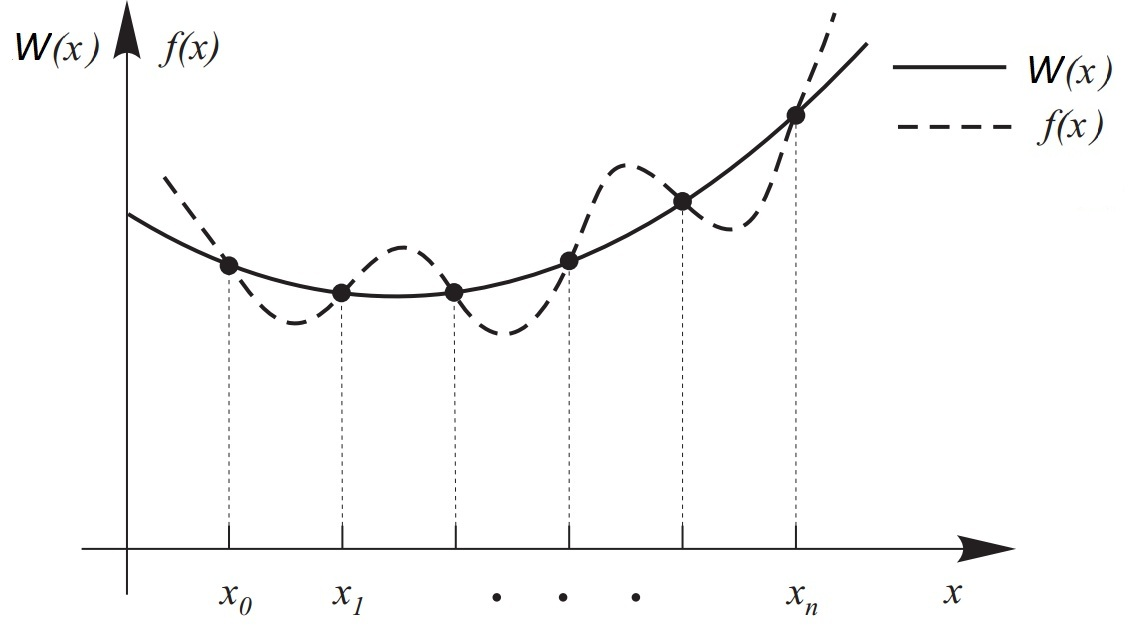
\includegraphics[scale=0.3]{R1.eps}
		\end{center}
	   \caption{\cite{klucz3} Funkcja interpolacyjna $W(x)$ oraz interpolowana $f(x)$ }
\label{R1}
\end{figure}

Maj�c ju� podstawy do tego, by wiedzie� czym jest interpolacja - przejd�my o krok dalej. Rozwa�my pewien liniowo niezale�ny uk�ad funkcji, zdefiniowanych na domkni�tym przedziale $[a,b]$:
\begin{equation}\label{funkcjeLiniowoNiezal}
	\phi_0(x),\phi_1(x),\ldots,\phi_n(x)
\end{equation}    
oraz zbi�r szukanych wsp�czynnik�w
\begin{equation}\label{wsp.AlphaDoKombinacjiLiniowej}
	\alpha_0,\alpha_1,\ldots,\alpha_n
\end{equation}
takich, �e ich kombinacja liniowa z (\ref{funkcjeLiniowoNiezal}) b�dzie spe�nia�a poni�szy uk�ad r�wna�:
\begin{equation}\label{KombinacjaLiniowaAlfaiPhi}
	\alpha_0\phi_0(x_i)+\alpha_1\phi_1(x_i)+\cdots+\alpha_n\phi_n(x_i)=f_i 
\end{equation}
gdzie $f_i\in F$ oraz $x_i \in X$. 

W \textit{interpolacji Lagrange'a} w sk�ad (\ref{funkcjeLiniowoNiezal}) wchodz� wielomiany okre�lone w nast�puj�cy spos�b:
\begin{equation}\label{i-TeFunkcjeBazoweLagrange'a}
	l_i(x)=\prod\limits_{j=0, j\neq i}^n  \frac{x-x_j}{x_i-x_j} \,\,\,\,\,\,\, (i=0,1,\ldots,n).
\end{equation}
S� one nazywane funkcjami bazowymi(wielomianami bazowymi) stopnia $n$. Warto zauwa�y�, �e zachodzi nast�puj�ca r�wno�� \cite{klucz3}: 
\begin{equation}\label{deltaKroneckera}
l_i(x_j)=\delta_{ij}=
					\left\{
							\begin{array}{lr}
							1, \,\,\,\,gdy\,\, i=j\\
							0, \,\,\,\,\,\,\,w p.p.
							\end{array}
					\right.
\end{equation}
Z powy�szego wynika, �e tylko w jednym przypadku $l_i(x)$ b�dzie mia�a warto�� r�n� od 0 (gdy $x=x_i$), zatem $\sum\limits_{i=0}^n l_i(x)=1$. Dodatkowo zauwa�my, �e macierz� charakterystyczn� uk�adu (\ref{KombinacjaLiniowaAlfaiPhi}) jest macierz jednostkowa. Skutkuje to tym, i� \cite{klucz2}
\begin{equation}\label{wielomianInterpolacyjnyLagrangea}
L_n(x)=\sum\limits_{i=0}^n f_i\cdot l_i(x)=\sum\limits_{i=0}^n f_i \prod\limits_{j=0, j\neq i}^n  \frac{x-x_j}{x_i-x_j}
\end{equation} 
b�dzie wielomianem o stopniu nie wi�kszym ni� $n$, oraz przyjmie warto�ci (\ref{f_i=f(x_i)})
w punktach w�z�owych. Wielomian (\ref{wielomianInterpolacyjnyLagrangea}) nazywany jest \textbf{wielomianem interpolacyjnym \textit{Lagrange'a}}. Z jego pomoc� w dosy� przyst�pny spos�b mo�emy interpolowa� dowoln� funkcj�.

\begin{ex}{(Wyznaczanie wielomianu interpolacyjnego \textit{Lagrange'a} stopnia $n=2$)}\label{Przyklad_WielomianInterpolacyjnyLagrangea1}\\\hfill
\textit{Zbudujemy wielomian interpolacyjny $L_2(x)$ dla funkcji $f(x)=e^{x^2}$ rozpatrywanej na ograniczonym przedziale $[0,1]$. 
%Kolejno oblicz $L_2(0,6)$ i wynik por�wnaj z warto�ci� rzeczywist� wiedz�c, �e $f(0,6)=e^{(0,6)^2}=1,4(3)$.
}

W celu wyznaczenia wielomianu \textit{Lagrange'a} stopnia $n=2$, potrzebowa� b�dziemy $n+1$ w�z��w takich, �e $a=x_0<x_1<x_2=b$. Przyjmijmy zatem nast�puj�ce ich warto�ci: 
$x_0=0$, $x_1=\frac{1}{2}$, $x_2=1.$ 
Korzystaj�c bezpo�rednio z r�wnania (\ref{wielomianInterpolacyjnyLagrangea}) dostajemy:
$$L_2(x)=f(x_0)\frac{(x-x_1)(x-x_2)}{(x_0-x_1)(x_0-x_2)}+
f(x_1)\frac{(x-x_0)(x-x_2)}{(x_1-x_0)(x_1-x_2)}+
f(x_2)\frac{(x-x_0)(x-x_1)}{(x_2-x_0)(x_2-x_1)}$$
Podstawiamy kolejno warto�ci w�z��w do r�wnania $L_2(x)$, otrzymuj�c wielomian interpoluj�cy nasz� funkcj� $f(x)=e^{x^2}$ na $[a,b]=[0,1]$:
$$L_2(x)=e^0\frac{(x-\frac{1}{2})(x-1)}{(0-\frac{1}{2})(0-1)}+
e^{(\frac{1}{4})} \frac{(x-0)(x-1)}{(\frac{1}{2}-0)(\frac{1}{2}-1)}+e^4\frac{(x-0)(x-\frac{1}{2})}{(1-0)(1-\frac{1}{2})}=
2,30046x^2-0,58218x+1$$
%Ostatecznie wyznaczamy warto�� $L_2(0,6)$:
%$$L_2(0,6)=2,30046\cdot(0,6)^2-0,58218\cdot(0,6)+1=1,4788576$$
%Warto�� interpolowana $L_2(0,6)$ odbiega nieco od warto�ci dok�adnej $f(0,6)$. 
\end{ex} 

Wyprowadzona w powy�szym przyk�adzie dla funkcji $f(x)$ i zadanych w�z��w posta� wielomianu $L_2(x)$ jest jednoznaczna. M�wi o tym nast�puj�ce twierdzenie:
\begin{theorem}{(O istnieniu i jednoznaczno�ci wielomianu interpolacyjnego \textit{Lagrange'a} )}\label{TwOJednoznacznosciWielomLagrangea}\\\hfill
Zadanie interpolacyjne \textit{Lagrange�a} ma zawsze dok�adnie jedno rozwi�zanie, kt�re mo�na wyrazi� wzorem (\ref{wielomianInterpolacyjnyLagrangea}). Oznacza to, �e dla dowolnej funkcji $f: X\rightarrow\re$ oraz jej warto�ci $f(x_i)$ w $n+1$ zadanych w�z�ach $x_i$ ($i=0,1,\ldots,n$), istnieje dok�adnie jeden wielomian $L_n(x)$ interpoluj�cy $f(x)$, dla kt�rego prawdziwa jest zale�no�� $L_n(x_i)=f(x_i)$.
\end{theorem}

%Przeprowad�my dow�d twierdzenia \ref{TwOJednoznacznosciWielomLagrangea}, by wykaza� jego s�uszno��.

\begin{dowod*}\label{DowodTwOJednoznacznosciWielomLagrangea}\hfill\\
Dowodzenie rozpoczniemy od wykazania faktu, �e rozwi�zanie w og�le istnieje.  Skonstruujmy je przy u�yciu  wielomian�w bazowych \textit{Lagrange'a} $l_i(x)$ z (\ref{i-TeFunkcjeBazoweLagrange'a}), oraz r�wnania (\ref{deltaKroneckera}). Nale�y zauwa�y�, �e odpowiadaj�ca dla ka�dego z w�z��w $x_i$, gdzie ($i=0,1,\ldots,n$) funkcja $l_i(x)$ jest wielomianem $n$-tego stopnia. W zwi�zku z tym \cite{klucz5}
$$L_n(x)=\sum\limits_{i=0}^n f(x_i)\cdot l_i(x)$$ 
b�dzie wielomianem stopnia co najwy�ej $n$. Ponadto odwo�uj�c si� do (\ref{deltaKroneckera}) powy�szy wz�r mo�emy przekszta�ci� do nast�puj�cej postaci:
$$L_n(x_j)=\sum\limits_{i=0}^n f(x_i)\cdot\delta_{ij}=f(x_j). $$
Wynika  st�d bezpo�rednio fakt, �e $L_n(x)$ jest wielomianem interpolacyjnym \textit{Lagrange'a}. Interpoluje on funkcj� $f(x)$ przy zadanych w�z�ach $x_i$ ($i=0,1,\ldots,n$). 

Kolejno poka�my, �e wyznaczany wielomian interpolacyjny \textit{Lagrange'a}  $L_n(x)$ jest zawsze jednoznaczny. Je�eli zapiszemy go w postaci pot�gowej (naturalnej) w bazie jednomian�w \(\{1, x, x^2, \dots, x^n, \ldots\}\) tzn.$$L_n(x)=\sum\limits_{i=0}^n a_i\cdot x^i,$$
to zauwa�amy, �e rozwi�zanie naszego problemu sprowadza si� do wyznaczenia $n+1$ wsp�czynnik�w $a_i$ ($i=0,1,\ldots,n$) takich, �e b�d� one spe�nia�y nast�puj�cy uk�ad $n+1$ r�wna� liniowych:
\begin{equation}\label{Dowod_UkladWPostaciMacierzowej}
\begin{bmatrix}
1 & x_0 & x_0^2 & x_0^3 & \cdots & x_0^n\\
1 & x_1 & x_1^2 & x_1^3 & \cdots & x_1^n\\
1 & x_2 & x_2^2 & x_2^3 & \cdots & x_2^n\\
\vdots & \vdots & \vdots & \vdots& \vdots& \vdots\\
1 & x_n & x_n^2 & x_n^3 & \cdots & x_n^n
 \end{bmatrix}
 \begin{bmatrix}
a_0\\
a_1\\
a_2\\
\vdots\\
a_n
 \end{bmatrix}
 =
  \begin{bmatrix}
  f(x_0)\\
f(x_1)\\
f(x_2)\\
\vdots\\
f(x_n)
 \end{bmatrix}
\end{equation}

Niech symbolicznym zapisem powy�szego uk�adu b�dzie $X \cdot A=F$. Macierz $X$ jest tak zwan� macierz� \textit{Vandermonde'a}. Zatem wiadomo, �e jej wyznacznik jest $\neq 0$, przy za�o�eniu, �e $x_0 \neq x_1\neq\ldots\neq x_{n-1}\neq x_n$. W zwi�zku z tym uk�ad (\ref{Dowod_UkladWPostaciMacierzowej}) posiada jednoznaczne rozwi�zanie, co ko�czy dow�d. $\square$
\end{dowod*}


Je�eli obliczyliby�my warto�� wielomianu interpolacyjnego  \textit{Lagrange'a} $L_2(x)$ (zbudowanego w przyk�adzie \ref{Przyklad_WielomianInterpolacyjnyLagrangea1}) dla pewnego $x$ nale��cego do dziedziny $f(x)$ i por�wnali j� z warto�ci� dok�adn� $f(x)$ dla tego samego argumentu, to zauwa�yliby�my, �e wynik jest obarczony pewnym b��dem. Nosi on miano \textit{b��du interpolacji}. Dla wielomian�w \textit{Lagrange'a} definiujemy go w nast�puj�cy spos�b:
\begin{definition}{(B��d interpolacji wielomianu \textit{Lagrange'a})}\\\hfill
We�my $$M_{n+1}=\sup\limits_{x\in[a,b]}|f^{(n+1)}(x)|$$  $$m_{n+1}=\sup\limits_{x\in[a,b]}|\omega_{n+1}(x)|,$$\\ przy czym \,$\omega_n(x)=(x-x_0)\ldots(x-x_n)=\prod\limits_{k=0}^n(x-x_k)$, za� $f(x)$ to funkcja interpolowana.\\
B��dem interpolacji wielomianu \textit{Lagrange'a} (stopnia $n$) nazywamy w�wczas takie
\begin{equation}\label{Bl�dInterpolacjiWielomLagrangea}
	\delta_L=\frac{M_{n+1}\cdot m_{n+1}}{(n+1)!},
\end{equation}
dla kt�rego zachodzi: $$|L_n(x)-f(x)|\leq\delta_L \,\,\,\,,x\in[a,b].$$

\end{definition}    

  
\section{Wielomiany \textit{Lagrange'a} dla funkcji dw�ch zmiennych}


\chapter{Kwadratury Newtona-Cotesa dla ca�ki pojedynczej}


Niech $f(x)$ b�dzie funkcj� zdefiniowan� na przedziale $[a,b]$ o warto�ciach rzeczywistych tzn. $f: [a,b]\rightarrow \re$. 
Rozwa�my pewn� ca�k� 
\begin{equation}\label{I(f)=Calkaf(x)}
I(f)=\int\limits_a^b f(x) dx
\end{equation}

Funkcj� podca�kow� zawsze mo�emy zast�pi� inn� funkcj� tak�, �e w miar� mo�liwo�ci poni�sze przybli�enie b�dzie prawdziwe:
\begin{equation}\label{ZastapienieFunkcjiFxfunkcjaGx}
\int\limits_a^b f(x) dx \approx \int\limits_a^b g(x) dx
\end{equation}

W praktyce cz�sto spotka� mo�emy si� z przypadkiem takim, ze do wyznaczenia przybli�onych warto�ci $I(f)$  stosowane s� wzory nazywane kwadraturami. 
Owe kwadratury opieraj� si� jedynie na warto�ciach $f(x)$ w punktach w�z�owych i mog� niezbyt dok�adnie przybli�a� wynik tzn: 
\begin{equation}\label{WzorKwadratura}
\int\limits_a^b f(x) dx \approx \sum\limits_{i=0}^n a_if(x_i),\,\,\,\, x_i\in[a,b],
\end{equation}
przy czym wsp�czynniki $a_i$ s� niezale�ne od $f(x)$ (nazywamy je wsp�czynnikami kwadratury), za� $x_i$ nosi miano w�z��w kwadratury.

Naszym celem jest jednak to, by jak najbardziej zminimalizowa� b��d pojawiaj�cy si� podczas przybli�ania warto�ci $I(f)$. W zwi�zku z tym mo�emy zastosowa� zabieg zast�pienia funkcji $f(x)$ w ca�ce $I(f)$ wielomianem interpoluj�cym j�. W tym celu wykorzystamy wielomian interpolacyjny \textit{Lagrange'a} (\ref{wielomianInterpolacyjnyLagrangea}). Po podstawieniu go do (\ref{WzorKwadratura}) otrzymamy:

\begin{equation}\label{SumaCalkowaLagrangeWkwadraturze}
\int\limits_a^b f(x) dx \approx \int\limits_a^b L_n(x) dx=
\sum\limits_{i=0}^n \alpha_i f(x_i) dx,
\end{equation}
gdzie 
\begin{equation}\label{wspolczynnikAi}
\alpha_i=\int\limits_a^b l_i(x),
\end{equation}
 natomiast 
 \begin{equation}\label{l_iDlaKwadraturN-C}
 l_i(x)=\prod\limits_{j=0, j\neq i}^n  \frac{x-x_j}{x_i-x_j} \,\,\,\,\,\,\, (i=0,1,\ldots,n).
 \end{equation}
W zwi�zku z powy�szym ca�k� (\ref{I(f)=Calkaf(x)}) mo�emy wyrazi� w nast�puj�cy spos�b:
\begin{equation}\label{PrzyblizenieCalkiSumaCalkowaZwielomianamiBazowymiLagrangea}
\int\limits_a^b f(x) dx \approx \sum\limits_{i=0}^n f(x_i)\int\limits_a^b l_i(x) dx
\end{equation}
Je�eli w (\ref{PrzyblizenieCalkiSumaCalkowaZwielomianamiBazowymiLagrangea}) rozpatrzymy tylko w�z�y takie, �e $x_0=a$, $x_n=b$, a ka�dy w�ze� po�redni le��cy pomi�dzy $x_0$ a $x_n$ jest postaci $x_i=a+ih$ $(i=0,1,\ldots,n)$, $h=\frac{x_n-x_0}{n}$, to kwadratur� tak� nazwiemy kwadratur� \textbf{Newtona-Cotesa}. Skupimy si� na rozwa�eniu trzech r�nych kwadratur tego typu, b�d� nimi: \textit{wz�r trapez�w}, \textit{wz�r Simpsona} oraz \textit{wz�r prostok�t�w}.


\section{Wz�r trapez�w}

%Zauwa�my, �e przybli�enie $\sum\limits_{i=0}^n f(x_i)\int\limits_a^b L_i(x) dx$ jest szczeg�lnym przypadkiem sumy z r�wnania (\ref{WzorKwadratura}), przy czym: 

%\begin{equation}\label{wspolczynnikAi}
%a_i=\int\limits_a^b L_i(x) dx
%\end{equation}


Do wyznaczenia wzoru trapez�w b�dziemy wykorzystywa� wielomian interpolacyjny \textit{Lagrange'a} rz�du $n=1$ ($L_1(x)$) utworzony dla w�z��w $a$ i $b$.
Zastosujmy w (\ref{l_iDlaKwadraturN-C}) nast�puj�ce podstawienie: $x=a+hs$. Warto�ci $a,h$ s� pewnymi sta�ymi, natomiast $s$ jest zmienn� niezale�n�.
$$l_i(x)=\prod\limits_{j=0, j\neq i}^n \frac{x-x_j}{x_i-x_j}=
\prod\limits_{j=0, j\neq i}^n \frac{a+hs-(a+jh)}{(a+ih)-(a+jh)}=
\prod\limits_{j=0, j\neq i}^n \frac{s-j}{i-j}$$
Otrzymujemy zatem:
\begin{equation}\label{WielomianLagrangeaPoPodstawieniuZaX}
l_i(x)=\prod\limits_{j=0, j\neq i}^n \frac{s-j}{i-j}=\psi_i(s)
\end{equation}
$\psi_i(s)$ to nasza nowa funkcja zmiennej $s$.


Ca�k� z r�wnania (\ref{wspolczynnikAi}) obliczymy metod� ca�kowania przez podstawienie. Skorzystamy z przedstawionego przed chwil� podstawienia $x=a+hs$ oraz r�wnania (\ref{WielomianLagrangeaPoPodstawieniuZaX})\\

$a_i=\int\limits_a^b l_i(x) dx=\left\{\begin{array}{ll}
x=a+hs\\
dx=h ds\\
b=a+hs \Rightarrow \frac{b-a}{h}=s\Rightarrow s=n\\
a=a+hs \Rightarrow 0=hs \Rightarrow s=0
\end{array}\right\}=h\int\limits_0^n \psi_i(s)ds
$\\

Chcemy wyliczy� teraz warto�ci wsp�czynnik�w kwadratury $a_0$ i $a_1$. Pami�tamy o tym, �e  do oblicze� wykorzystujemy posta� wielomianu \textit{Lagrange'a} rz�du $n=1$, zatem b�dziemy ca�kowali w granicach $[0,n]=[0,1]$
$$a_0=h\int\limits_0^1 \phi_0(s) ds=h\int\limits_0^1\frac{s-1}{0-1}ds=\int\limits_0^1(1-s)ds= h\left[s-\frac{s^2}{2}\right]_0^1=\frac{h}{2}$$
$$a_1=h\int\limits_0^1 \phi_1(s) ds=h\int\limits_0^1\frac{s-0}{1-0}ds=\int\limits_0^1(s)ds= h\left[\frac{s^2}{2}\right]_0^1=\frac{h}{2}$$
Po wstawieniu wyliczonych wsp�czynnik�w do (\ref{WzorKwadratura}) otrzymujemy 
\begin{equation}\label{wzorTrapezowBrakPodzialu}
\begin{array}{cc}
\int\limits_a^b f(x) dx \approx \sum\limits_{i=0}^1 a_if(x_i)=a_0f(x_0)+a_1f(x_1)=\\
=\frac{h}{2}f(x_0)+\frac{h}{2}f(x_1)=\frac{h}{2}(f(x_0)+f(x_1))
\end{array}
\end{equation}
Wz�r ten nazywamy \textbf{wzorem trapez�w}. Zauwa�my, �e suma wsp�czynnik�w $\alpha_0$,$\alpha_1$ jest r�wna $h\cdot n$. W p�niejszych podrozdzia�ach r�wnie� zetkniemy si� z tak� prawid�owo�ci� rozpatruj�c wy�szy rz�d wielomian�w \textit{Lagrange'a} dla $n>1$.
%Gdyby�my wyliczali wsp�czynniki dla $n=2$, to otrzymaliby�my wz�r \textit{Simpsona}

Podczas wyznaczania (\ref{wzorTrapezowBrakPodzialu}) przyj�li�my, �e przedzia� ca�kowania nie zosta� podzielony, a jedynymi w�z�ami by�y jego pocz�tek i koniec. W rzeczywisto�ci rozpatrujemy przypadki z wielokrotnym podzia�em przedzia�u. %Dzieje si� tak, poniewa� im wi�cej podzia��w dokonamy tym dok�adniejszy b�dzie uzyskany wynik. 
Je�eli przedzia� ca�kowania $[a,b]$ podzielimy na $\geq 2$ r�wne cz�ci takie, �e $a=x_0<x_1<\ldots<x_n=b$, to wz�r przyjmie posta�:
\begin{equation}\label{OgolnyWzorTrapezow}
\begin{array}{cc}
\int\limits_a^b f(x)dx=\sum\limits_{i=0}^{n-1}\int\limits_{x_i}^{x_{i+1}}f(x)dx\approx\\ \approx(\frac{h}{2}(f(x_0)+f(x_1))+\cdots+\frac{h}{2}(f(x_{n-1})+f(x_n)))=\\
=\frac{h}{2}(f(x_0)+2f(x_1)+\cdots+2f(x_{n-1})+f(x_n))=\\ 
=\frac{h}{2}\sum\limits_{i=0}^{n-1}[f(x_i)+f(x_{i+1})]
\end{array}
\end{equation}


W wyprowadzonym powy�ej wzorze trapez�w (jak sama nazwa sugeruje) przybli�amy warto�� ca�ki sumuj�c pola trapez�w o ustalonej wysoko�ci $h$ (odleg�o�� pomi�dzy kolejnymi w�z�ami) i podstawach o d�ugo�ci $f(x_i)$ i $f(x_{i+1})$ dla $i=0,1,\ldots,n-1$. Rysunek \ref{R1} z pewno�ci� pomo�e nam lepiej zrozumie� zagadnienie, na kt�rym si� skupiamy.
\begin{figure}[H]
		\begin{center}
		\includegraphics[scale=0.13]{R2.eps} 
		\end{center}
	   \caption{Graficzne przedstawienie idei zastosowania wzoru trapez�w do ca�kowania}
\label{R1}
\end{figure}

Przejd�my do praktycznego zastosowania wzoru (\ref{OgolnyWzorTrapezow}) w celu pokazania jego przydatno�ci. Obliczenia dla zadanej funkcji przeprowadzimy r�cznie przy relatywnie ma�ej liczbie podzia�u przedzia��w, oraz wykorzystuj�c procedur� stworzon� w j�zyku \textit{Maple} dla du�o wi�kszej liczby podzia�u. 


\begin{ex}{(Wyznaczanie przybli�onej warto�ci ca�ki przy wykorzystaniu wzoru trapez�w)}\label{PrzykladCalkaPojedynczaMetodaTrapezow}\hfill
\textit{Wyznaczy� przybli�on� warto�� ca�ki $\int\limits_0^{\frac{3}{2}} e^{x^2} dx$ przyjmuj�c, �e przedzia� ca�kowania dzielimy na n=6 r�wnych cz�ci(7 w�z��w)}\\

Do rozwi�zania zadania skorzystamy z og�lnego wzoru trapez�w. Wyznaczamy warto�ci w�z��w oraz odleg�o� $h=\frac{b-a}{n}$ pomi�dzy kolejnymi w�z�ami:\\
$h=\frac{\frac{3}{2}-0}{6}=\frac{1}{4}$, $x_0=0$, $x_1=\frac{1}{4}$, $x_2=\frac{2}{4}$, $x_3=\frac{3}{4}$, $x_4=1$, $x_5=\frac{5}{4}$, $x_6=\frac{6}{4}$.\\ 
Wyliczone warto�ci wstawiamy do (\ref{OgolnyWzorTrapezow}):
\begin{center}
$\int\limits_0^{\frac{3}{2}} e^{x^2} dx=\frac{\frac{1}{4}}{2}(f(x_0)+2f(x_1)+2f(x_2)+2f(x_3)+2f(x_4)+2f(x_5)+f(x_6))=$\\
$=\frac{1}{8}(e^0+2e^{{(\frac{1}{4})}^2}+2e^{{(\frac{2}{4})}^2}+2e^{{(\frac{3}{4})}^2}+2e^1+2e^{{(\frac{5}{4})}^2}+e^{{(\frac{6}{4})}^2})\approx 
\frac{1}{8}(1+2\cdot 1,06449+2\cdot 1,28402+2\cdot 1,75505+2\cdot  2,71828+2\cdot 4,77073+9,48773)\approx 4,20911$\\
\end{center}
Warto�� dok�adna wynosi w zaokr�gleniu $4,063114$. Jak wida� r�nica w wyniku jest dosy� znacz�ca przy ustalonych warto�ciach w�z��w, poniewa� otrzymany przez nas wynik to $4,20911$.
\end{ex}


Z regu�y im wi�cej podzia��w przedzia�u wykonamy, tym dok�adniejsze powinni�my otrzymamy przybli�enie. Mo�na wnioskowa� w ten spos�b r�wnie� poddaj�c si� na analizie wzoru na b��d metody trapez�w (im wi�kszy $n$ tym mniejsza warto�� $\delta_T$):
\begin{definition}{(B��d przybli�enia wzorem trapez�w)}\\\hfill
Niech $f: [a,b]\rightarrow \re$ b�dzie klasy $C^2$ na $[a,b]$, oraz niech $n$ wyznacza ilo�� podzia��w tego przedzia�u, to b��d metody trapez�w wyra�a nast�puj�cy wz�r: 
\begin{equation}\label{BladMetodyTrapezow}
\delta_T = \frac{(b-a)^3}{12n^2} \cdot M_2,
\end{equation}
gdzie 
\begin{equation}\label{CzynnikM2DoBleduMetodyTrapezow}
M_2= \sup_{x \in [a,b]} \, | f^{''}(x) |
\end{equation}

\end{definition}
Sprawdzimy jednak s�uszno�� naszego twierdzenia wykorzystuj�c do tego stworzon� na nasze potrzeby procedur� w j�zyku Maple. Pos�u�y nam ona do zautomatyzowania procesu obliczania przybli�onych warto�ci ca�ek oznaczonych metod� trapez�w:

\begin{proc}{(Procedura wyznaczaj�ca warto�ci ca�ek pojedynczych metod� trapez�w)}\label{MAPLE_MetodaTrapezowCalkaPojedyncza}
\begin{verbatim}
> trapez:=proc(a,b,N) 
local h,j,k,x,y,t,tp; 
h:=(b-a)/N; 
for j from 0 to N do x:= j -> a+j*h od;  
for j from 0 to N do y:= j -> f(x(j)) od;  
t:= h/2 * sum(y(k)+y(k+1), k=0..N-1); 
tp:=evalf(t,12); 
end;
\end{verbatim}
\end{proc}

\hspace{-1cm}{Przed przej�ciem do prezentacji wynik�w jakie zwr�ci powy�sza procedura, nale�y wyja�ni� nieco jej zasad� dzia�ania i znaczenie parametr�w.}

\hspace{-1cm}{Pierwsza linia jest deklaracj� procedury \textit{trapez} z nast�puj�cymi parametrami wej�ciowymi:}\\
\textbf{a}, \textbf{b} - s� odpowiednio dolnym i g�rnym kra�cem przedzia�u ca�kowania\\
\textbf{N} - okre�la liczb� podprzedzia��w na kt�re podzielony zostanie nasz przedzia� $[a,b]$\\
Kolejno deklarujemy zmienne pomocnicze z kt�rych korzysta procedura ( nie pobierane od u�ytkownika) oraz wyznaczamy warto�� kroku $h$, czyli odleg�o�� pomi�dzy dwoma kolejnymi w�z�ami. Nast�pnie wyznaczamy wszystkie w�z�y na danym przedziale oraz wyliczamy warto�ci (deklarowanej przed wywo�ywaniem procedury) funkcji $f$ w tych�e w�z�ach. Przedostatni krok polega na zsumowaniu wyliczonych przed chwil� warto�ci w spos�b zgodny ze wzorem (\ref{OgolnyWzorTrapezow}). Algorytm ko�czymy poprzez przekszta�cenie sumy do "przyjaznej" \,postaci i prezentacj� wyniku z dok�adno�ci� do 12 miejsc po przecinku. 


Poni�sza tabela prezentuje wyniki procedury  \ref{MAPLE_MetodaTrapezowCalkaPojedyncza} (ozn. $W_{trapez}$) dla coraz to wi�kszej liczby podprzedzia��w $N$. Uwzgl�dniono w niej r�wnie� warto�ci b��d�w wzoru trapez�w (ozn. $\delta_T$) wyliczone zgodnie ze wzorem (\ref{BladMetodyTrapezow}) oraz modu�  r�nicy pomi�dzy warto�ci� dok�adn� ca�ki a otrzyman� w ramach test�w procedury (ozn. $|W-W_{trapez}|$). Do kalkulacji wykorzystamy funkcj� z przyk�adu \ref{PrzykladCalkaPojedynczaMetodaTrapezow} oraz podan� w rozwi�zaniu informacj� na temat przybli�onej do 6 miejsca po przecinku warto�ci dok�adnej ca�ki $\int\limits_0^{\frac{3}{2}} e^{x^2} dx\approx 4,063114$.  \\

\begin{table}[h!]
\label{WynikiZProceduryTrapez}
\centering
 \begin{tabular}{|c|c|c|c|} 
 \hline
 $\mathbf{N}$ & $\mathbf{W_{trapez}}$ &$\mathbf{\delta_T}$& $\mathbf{|W-W_{trapez}|}$  \\ [0.5ex] 
 \hline \hline
 6 &  &  &  \\ 
 \hline
 30&  &  & \\
 \hline 
 100&  &  &  \\
 \hline 
 200&  &  &  \\
 \hline 
 400&  &  & \\ 
  \hline 
 800&  &  & \\
  \hline 
 1200&  &  & \\
  \hline 
 2000&  &  & \\
  \hline 
 5000&  &  & \\[0.5ex] 
 \hline 
 \end{tabular}
\end{table}

-------------DODAC:  por�wna� wyniki otrzymane metod� trapez�w dla n=6 liczone recznie i dla duzego n liczonego procedur�, pokaza� ze im wi�ksza liczba podzia��w tym dok�adniejszy wynik, pokaza� ze mozna wyliczy� minimaln� liczb� podzia�u przedzia��w by otrzyma� wynik z maksymalnie okreslonym bledem-------- 




\section{Wz�r Simpsona}
\section{Wz�r prostok�t�w}


\chapter{Kwadratury Newtona-Cotesa dla ca�ek podw�jnych w prostok�cie}
W ca�ym poprzednim rozdziale skupiali�my si� na metodach ca�kowania numerycznego. Odnosi�y si� one jednak tylko do funkcji jednej zmiennej - zatem ca�kowanie odbywa�o si� na pewnym przedziale domkni�tym. Teraz chcemy poszerzy� nasz� wiedz� i przej�� o jeden krok dalej. Nasze rozwa�ania zostan� skierowane ponownie na te same, co poprzednio metody ca�kowania numerycznego. Znacz�ca r�nica polega�a b�dzie na tym, �e zajmiemy si� ca�kowaniem funkcji dw�ch zmiennych. Wszystkie nasze dzia�ania maj� na celu wy�onienie najdok�adniejszej metody wyznaczania warto�ci ca�ek podw�jnych przy pomocy prezentowanych algorytm�w.  W badaniach wyr�nimy dwa typy obszar�w ca�kowania, b�d� to:
\begin{itemize}
\item[a)] Obszar normalny ze wzgl�du na zmienn� $x$ i $y$
\item[b)] Obszar normalny tylko ze wzgl�du na zmienn� $x$
\end{itemize}

W celu kontynuacji rozwa�a� musimy przypomnie� niezb�dn� dla nas definicj� normalno�ci obszaru:
\begin{definition}(Obszar normalny)\\
O obszarze normalnym w przestrzeni kartezja�skiej $\re ^2$ 
\begin{itemize}
\item[a)]\label{ObszaryNormalneOx}wzgl�dem osi $OX$ (tj. wzgl�dem $x$) m�wimy, gdy podzbi�r p�aszczyzny kartezja�skiej ograniczony jest przez wykresy pewnych dw�ch funkcji ci�g�ych $u(x)$ i $v(x)$ oraz dwie proste r�wnoleg�e do osi $OY$.    
\item[b)]\label{ObszaryNormalneOy}wzgl�dem osi $OY$ (tj. wzgl�dem $y$) m�wimy, gdy podzbi�r p�aszczyzny kartezja�skiej jest wyznaczany poprzez wykresy dw�ch r�nych funkcji ci�g�ych $l(y)$ i $k(y)$ oraz dwie proste, kt�re s� r�wnoleg�e do osi $OX$.
\item[c)]ze wzgl�du na zmienne $x$ i $y$ m�wimy, gdy podzbi�r p�aszczyzny kartezja�skiej jest ograniczony przez dwie proste r�wnoleg�e do osi $OX$ oraz dwie proste r�wnoleg�e do $OY$ 

\end{itemize}

\section{Wz�r trapez�w }\label{Rozdzial3.1_WzorTrapezow2DObszNormalny}
W podrozdziale \ref{Podrozdzial_WzorTrapezow} wyprowadzili�my ju� wz�r trapez�w (\ref{wzorTrapezowBrakPodzialu}) i uog�lniony wz�r trapez�w (\ref{OgolnyWzorTrapezow}). Najbardziej interesuje nas drugi ze wspomnianych. Istnieje mo�liwo�� rozszerzenia go na przypadek og�lny dotycz�cy funkcji dw�ch zmiennych. Zbadajmy wariant, dla kt�rego obszar ca�kowania jest normalny ze wzgl�du na dwie zmienne.  

Niech ca�kowanie odbywa si� na obszarze $\Omega=\{a\leq x\leq b ; c\leq y \leq d \}$. 
Przedzia� $[a,b]$ zostanie podzielony na $n$ podprzedzia��w postaci $[x_i,x_{i+1}]$ ($i=0,1,\ldots, n-1$). Podobnie b�dzie dla $[c,d]$, podzielimy go na $m$ podprzedzia��w $[y_j,y_{j+1}]$ ($j=0,1,\ldots, m-1$). \mbox{W zwi�zku} z tym zajdzie nast�puj�ca prawid�owo��:
\vspace{-0.5cm}\begin{equation}\label{WezlyTrapez2}
\begin{array}{cc}
a=x_0\leq x_1\leq x_2\ldots\leq x_n=b \\
c=y_0\leq y_1\leq y_2\ldots\leq y_m=d \\
\end{array}
\end{equation} 
Posta� punkt�w $x_i$, $y_j$ nale��cych do tych przedzia��w, jak r�wnie� krok�w $h_x$ i $h_y$ pomi�dzy kolejnymi warto�ciami w�z��w to:
\vspace{-0.5cm}\begin{equation}\label{WezlyNaObszarzeProstokatnymTrapez2}
\begin{array}{cc}
x_i=x_0+ih_x,\,\,\,\, h_x=\frac{b-a}{n} \,\,\,\,(i=0,1,\ldots ,n)\\
y_j=y_0+jh_y, \,\,\,\,h_y=\frac{d-c}{m} \,\,\,\,(j=0,1,\ldots ,m)\\
\end{array}
\end{equation}

Zapiszmy wz�r (\ref{OgolnyWzorTrapezow}) w nieco innej postaci, kt�ra b�dzie dla nas bardziej por�czna, tzn.:
\begin{equation}\label{UogolnionyWzorTrapezow1Przeksztalcony}
\int\limits_a^b f(x) dx \approx \frac{h}{2}\sum\limits_{i=0}^{n-1}[f(x_i)+f(x_{i+1})]=\frac{h}{2}\left[f(x_0)+f(x_n)+2\sum\limits_{i=1}^{n-1} f(x_i) \right].
\end{equation} 
Kolejno we�my pewn� oznaczon� ca�k� podw�jn� postaci \cite{klucz11}:
\begin{equation}\label{CalkaPodwojna}
I_{T2}=\int\limits_a^b\int\limits_c^d f(x,y)dydx=\int\limits_a^b g(x)dx\,\, ,
\end{equation} 
\end{definition}
\begin{flushleft}
przy czym ( rozbudowuj�c (\ref{UogolnionyWzorTrapezow1Przeksztalcony}) o dodatkow� zmienn�\,)
\end{flushleft}
\begin{equation}\label{Wyjasnienie_g(x)_metodaTrapezow2}
g(x)=\int\limits_c^d f(x,y)dy\approx\frac{h_y}{2}\left[ f(x,y_0)+f(x,y_m)+2\sum\limits_{j=1}^{m-1}f(x,y_j)\right].
\end{equation}   
Podstawmy opisan� przez r�wnanie (\ref{Wyjasnienie_g(x)_metodaTrapezow2}) posta� $g(x)$ do (\ref{CalkaPodwojna}). Zaskutkuje to tym, �e:
\begin{equation}\label{SprowadzenieCalkiPodwDoPojedynczejZSumaTrapez2}
I_{T2}=\int\limits_a^b\int\limits_c^d f(x,y)dydx\approx\int\limits_a^b \frac{h_y}{2}\left[ f(x,y_0)+f(x,y_m)+2\sum\limits_{j=1}^{m-1}f(x,y_j)\right] dx  \,.
\end{equation}
W celu wyeliminowania potrzeby ca�kowania w (\ref{SprowadzenieCalkiPodwDoPojedynczejZSumaTrapez2}) ponownie zostaje zastosowana metoda trapez�w z r�wnania (\ref{UogolnionyWzorTrapezow1Przeksztalcony}) (rozszerzona w podobny spos�b jak w (\ref{Wyjasnienie_g(x)_metodaTrapezow2})). Tym razem traktujemy $x$ jako zmienn�, natomiast ca�e wyra�enie podca�kowe jako jedn� funkcj�. Sprowadza to nasz problem do nast�puj�cego przypadku \cite{klucz11}
\begin{equation}\label{CalkaPodwojnaJakoSumaTrapez2}
\begin{array}{cc}
I_{T2}\approx \frac{h_x}{2} \left\lbrace \frac{h_y}{2}\left[ f(x_0,y_0)+f(x_0,y_m)+2\sum\limits_{j=1}^{m-1}f(x_0,y_j)\right] \right.\\
+ \frac{h_y}{2}\left[ f(x_n,y_0)+f(x_n,y_m)+2\sum\limits_{j=1}^{m-1}f(x_n,y_j)\right] \\
+ \left. 2\sum\limits_{i=1}^{n-1}\frac{h_y}{2}\left[ f(x_i,y_0)+f(x_i,y_m)+2\sum\limits_{j=1}^{m-1}f(x_i,y_j)\right]
\right\rbrace
\end{array}
\end{equation}
Po uproszczeniu ostateczn� form� (\ref{CalkaPodwojnaJakoSumaTrapez2}) jest:
\begin{equation}\label{UogolnionyWzorTrapezow2_obszarNormalny}
\begin{array}{cc}
I_{T2}\approx \frac{h_x h_y}{4}\left\lbrace f(x_0,y_0)+f(x_0,y_m)+f(x_n,y_0)+f(x_n,y_m)
+ 4\sum\limits_{i=1}^{n-1}\sum\limits_{j=1}^{m-1}f(x_i,y_j)\right.\\
\left. +2\sum\limits_{j=1}^{m-1}\left[f(x_0,y_j)+f(x_n,y_j)\right]
+ 2\sum\limits_{i=1}^{n-1}\left[f(x_i,y_0)+f(x_i,y_m)\right]\right\rbrace
\end{array}
\end{equation}

Interesuj�cym faktem jest to, �e wsp�czynniki wagowe kwadratury opisanej powy�szym wzorem rozk�adaj� si� wed�ug pewnego schematu. Co oznacza, �e je�eli rozpisaliby�my (\ref{UogolnionyWzorTrapezow2_obszarNormalny}) tak, by uwzgl�dni� w nim wszystkie punkty w�z�owe postaci $(x_i,y_j)$ ( $i=0,1,\ldots,n$,\, \mbox{$j=0,1,\ldots,m$} ) nale��ce do pewnego obszaru prostok�tnego i spe�niaj�ce (\ref{WezlyNaObszarzeProstokatnymTrapez2}), to odpowiednio warto�ci przy kolejnych $f(x_i,y_j)$ ( $i=0,1,\ldots,n\,\,\,,\,\,\,\, j=0,1,\ldots,m$ ) rozk�ada�yby si� nast�puj�co \cite{klucz12}:
\begin{equation}\label{MacierzWspolczynnikowTrapez2}
\left[
\begin{array}{ccccccccc}
1 & 2 & 2 & 2 &\cdots & 2& 2& 2& 1\\
2 & 4 & 4 & 4 &\cdots & 4& 4& 4& 2\\
2 & 4 & 4 & 4 &\cdots & 4& 4& 4& 2\\
\vdots &\vdots &\vdots &\vdots & \ddots &\vdots &\vdots &\vdots &\vdots \\
2 & 4 & 4 & 4 &\cdots & 4& 4& 4& 2\\
1 & 2 & 2 & 2 &\cdots & 2& 2& 2& 1\\
\end{array}
\right]
\end{equation}
Powy�sza macierz znacz�co upraszcza i przyspiesza rozpisywanie \textbf{uog�lnionego wzoru trapez�w dla ca�ek podw�jnych po obszarach normalnych}. Dla przypadku uog�lnionego wzoru trapez�w dla ca�ki pojedynczej schemat ten ogranicza� si� jedynie do pierwszego wiersza (numeracja $i$ - od lewej do prawej, $j$ - od g�ry do do�u).

Obliczanie warto�ci ca�ki podw�jnej metod� trapez�w mo�emy sprowadzi� r�wnie� do  sumowania obj�to�ci pewnych bry� trapezoidalnych. Innymi s�owy - rozwa�my podzia� obszaru ca�kowania $\Omega = [a,b] \times [c,d]$ na $n\cdot m$ podobszar�w, co prezentuje rysunek \ref{R4} zamieszczony poni�ej:

\begin{figure}[H]
		\begin{center}
		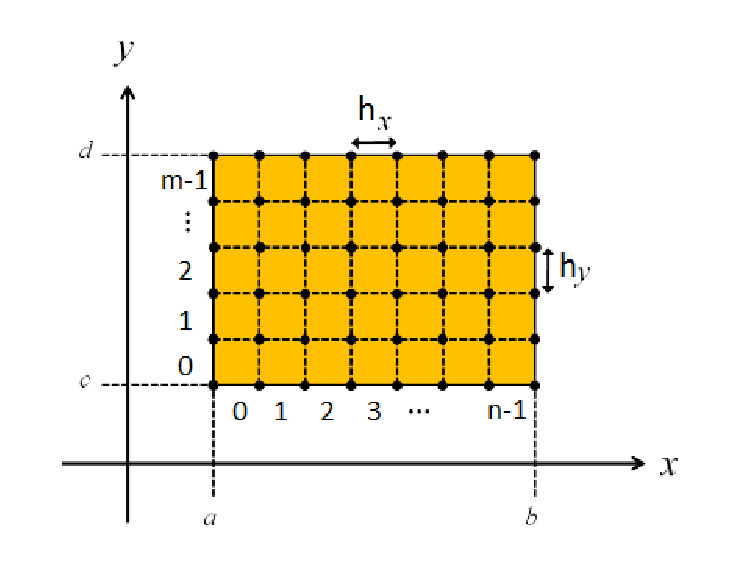
\includegraphics[scale=0.7]{R4.eps}
		\end{center}
	   \caption{\cite{klucz10} Metoda trapez�w dla ca�ek podw�jnych - podzia� obszaru ca�kowania na podobszary }
\label{R4}
\end{figure}
\begin{flushleft}
Jak wida�, ka�dy z podobszar�w jest wyznaczany przez cztery wierzcho�ki $(x_i,y_j)$ (definicja $x_i$, $y_j$ taka jak w (\ref{WezlyNaObszarzeProstokatnymTrapez2})). Do obliczenia obj�to�ci ka�dej z takich bry� trapezoidalnych potrzebne s� nam pola podstawy ( ju� je znamy - s� one takie same dla ka�dego podobszaru i wynosz� $h_xh_y$), oraz odpowiadaj�ce dla nich wysoko�ci. Te ostatnie okre�limy jako �rednia arytmetyczna warto�ci funkcji $f(x,y)$ w czterech wierzcho�kach definiuj�cych ka�dy z podobszar�w ca�kowania. Ostatecznie obj�to�� ka�dej bry�y definiowa� b�dzie nast�puj�cy wz�r \cite{klucz10}:
\end{flushleft}
\begin{equation}\label{ObjetoscDowolnegoTrapezoiduMetodaTrapezow2}
T2V_{i,j}=h_xh_y\left[\frac{f(x_{i},y_{j})+f(x_{i+1},y_{j})+f(x_{i},y_{j+1})+f(x_{i+1},y_{j+1})}{4}\right],
\end{equation}
przy czym $h_x$, $h_y$ opisane s� w (\ref{WezlyNaObszarzeProstokatnymTrapez2}).\\ Rozszerzaj�c r�wnanie (\ref{ObjetoscDowolnegoTrapezoiduMetodaTrapezow2}), charakteryzuj�ce pojedyncz� obj�to�� bry�y na ca�y obszar ca�kowania dobrn�liby�my do r�wno�ci postaci  (\ref{UogolnionyWzorTrapezow2_obszarNormalny}). Analizuj�c powy�sze zapiski wnioskujemy i� zachodzi nast�puj�ca prawid�owo��: 
\begin{equation}\label{RownoscUogWzoruTrapezow2IWzoruZObjetosciami}
I_{T2V} = I_{T2}\approx \sum\limits_{i=0}^{n-1} \sum\limits_{j=0}^{m-1} h_xh_y\left[\frac{f(x_{i},y_{j})+f(x_{i+1},y_{j})+f(x_{i},y_{j+1})+f(x_{i+1},y_{j+1})}{4}\right]
\end{equation}
Por�wnuj�c macierz (\ref{MacierzWspolczynnikowTrapez2}) z rysunkiem \ref{R4} zauwa�ymy, �e elementy macierzy odzwierciedlaj� ilo�� podobszar�w, na styku kt�rych umiejscowiony zosta� dany w�ze�. Mo�na to te� traktowa� jako informacj� ilu krotnie dany punkt w�z�owy zostaje uwzgl�dniony podczas sumowania w (\ref{RownoscUogWzoruTrapezow2IWzoruZObjetosciami}).

Wz�r (\ref{UogolnionyWzorTrapezow2_obszarNormalny}) podobnie jak dla przypadku ca�ki pojedynczej mo�na r�wnie� otrzyma� wykorzystuj�c wielomiany \textit{Lagrange'a $L_{1,1}(x,y)$}. Podamy jedynie zarys przekszta�ce�, kt�re doprowadzi�yby nas do wyniku: 
\begin{equation}\label{WzorTrapezowWielomianemL11}
\begin{array}{cc}
I_{T2L} = \int\limits_a^b \int\limits_c^d f(x,y) dydx\approx \int\limits_a^b \int\limits_c^d L_{1,1}(x,y) dydx = 
\sum\limits_{i=0}^{n-1} \sum\limits_{j=0}^{m-1}\int\limits_{x_i}^{x_{i+1}} \int\limits_{y_j}^{y_{j+1}} L_{1,1}(x,y) dydx =\\
\frac{h_xh_y}{4} \sum\limits_{i=0}^{n-1} \sum\limits_{j=0}^{m-1} \left[f(x_{i},y_{j})+f(x_{i+1},y_{j})+f(x_{i},y_{j+1})+f(x_{i+1},y_{j+1})\right]
\end{array}
\end{equation}
Ostatnie przej�cie mog�o zosta� wykonane, poniewa� wynik dla ka�dej ca�ki $\int\limits_{x_i}^{x_{i+1}} \int\limits_{y_j}^{y_{j+1}} L_{1,1}(x,y) dydx$ jest takiej samej postaci, zmienia si� jedynie numer w�z�a branego pod uwag�. Dla przyk�adu:
\begin{equation}
\begin{array}{cc}
\int\limits_{x_0}^{x_{1}} \int\limits_{y_0}^{y_{1}} L_{1,1}(x,y) dydx
 =
 \int\limits_{x_0}^{x_{1}} \int\limits_{y_0}^{y_{1}}\left( f(x_0,y_0)\left(\frac{x-x_1}{x_0-x_1}\frac{y-y_1}{y_0-y_1} \right)
 +f(x_0,y_1)\left(\frac{x-x_1}{x_0-x_1}\frac{y-y_0}{y_1-y_0} \right)\right.\\
\left. +f(x_1,y_0)\left(\frac{x-x_0}{x_1-x_0}\frac{y-y_1}{y_0-y_1} \right)
 +f(x_1,y_1)\left(\frac{x-x_0}{x_1-x_0}\frac{y-y_0}{y_1-y_0} \right)
 \right) dydx= \ldots =\\ 
 \frac{h_xh_y}{4}\left[f(x_{0},y_{0})+f(x_{1},y_{0})+f(x_{0},y_{1})+f(x_{1},y_{1})\right]
\end{array}
\end{equation}

Jak wida� istnieje wiele sposob�w na to, by wyprowadzi� po��dany przez nas dwuwymiarowy wz�r trapez�w. Naj�atwiejsza do zrozumienia i p�niejszego zaimplementowania okazuje si� na pierwszy rzut oka jego posta� z r�wno�ci (\ref{RownoscUogWzoruTrapezow2IWzoruZObjetosciami}).\\ 
\newpage
Zechciejmy teraz wykorzysta� zdobyt� wiedz� w praktyce rozwi�zuj�c pewien przyk�ad.

\begin{ex}(Wyznaczanie warto�ci ca�ki podw�jnej wzorem trapez�w)\\
\textit{Wyznaczymy warto�� przybli�on� $\int\limits_0^{\frac{1}{2}}\int\limits_{\frac{1}{2}}^1 \frac{x+y}{x^2+y^2} dydx$ przy u�yciu uog�lnionego wzoru trapez�w dla ca�ek podw�jnych po obszarach normalnych. Przyjmijmy, �e przedzia�y ca�kowania dla obydwu zmiennych dzielimy na $n=m=2$ r�wne podprzedzia�y. }\\
Zgodnie z przyj�tymi za�o�eniami podzia� wygl�da nast�puj�co:
\begin{center}
$x_0=0 , x_1=\frac{1}{4} , x_2=\frac{1}{2} $\\
$y_0=\frac{1}{2} , y_1=\frac{3}{4} , y_2=1 $.\\
\end{center}
Warto�ciami krok�w pomi�dzy kolejnymi w�z�ami s�: $h_x=\frac{x_2-x_0}{2}=\frac{1}{4}$, $h_y=\frac{y_2-y_0}{2}=\frac{1}{4}$.

Przejd�my teraz do g��wnych rachunk�w prowadz�cych do wyniku, mianowicie:
\begin{center}
$\int\limits_0^{\frac{1}{2}}\int\limits_{\frac{1}{2}}^1 \frac{x+y}{x^2+y^2} dydx \approx
\frac{h_xh_y}{4}\left( f(x_0,y_0) + f(x_0,y_2) + f(x_2,y_0) + f(x_2,y_2)  + \right.$
$\left. + 4 f(x_1,y_1) + 2 f(x_0,y_1) + 2 f(x_2,y_1)+ 2 f(x_1,y_0) + 2 f(x_1,y_2)\right)=$
$=\frac{\frac{1}{16}}{4}\left( f(0,\frac{1}{2}) + f(0,1) + f(\frac{1}{2},\frac{1}{2}) + f(\frac{1}{2},1)  + \right.$
$\left. + 4 f(\frac{1}{4},\frac{3}{4}) + 2 f(0,\frac{3}{4}) + 2 f(\frac{1}{2},\frac{3}{4})+ 2 f(\frac{1}{4},\frac{1}{2}) + 2 f(\frac{1}{4},1)\right)=$\\
$=\frac{1}{64}\left(\frac{\frac{1}{2}}{\frac{1}{4}}+\frac{1}{1}+\frac{1}{\frac{2}{4}}+\frac{\frac{3}{2}}{\frac{5}{4}}+4 \frac{1}{\frac{10}{16}}+2\frac{\frac{3}{4}}{\frac{9}{16}}+2\frac{\frac{5}{4}}{\frac{13}{16}}+2\frac{\frac{3}{4}}{\frac{5}{16}}+2\frac{\frac{5}{4}}{\frac{17}{16}} \right)=$\\
$=\frac{1}{64}\left( 2+1+2+\frac{12}{10}+\frac{64}{10}+\frac{48}{18}+\frac{80}{26}+\frac{48}{10}+\frac{80}{34}\right)=0,398383295625$\\
\end{center}

Wynik dok�adny otrzymany przy wykorzystaniu zaawansowanego narz�dzia matematycznego wynosi $0,399181467986$. Bardzo szybko mo�emy zauwa�y�, �e b��d wzgl�dny (oznaczmy go jako \textbf{BW}) nie jest znacz�cy i wynosi zaledwie $0,2\%$ : 
\begin{center}
$BW = \frac{|0,399181467986 - 0,398383295625|}{0,399181467986} * 100\% \approx 0,19995\%\approx 0,2\% $ \\
\end{center}
Mo�emy zatem bezwzgl�dnie stwierdzi�, �e otrzymany wynik jest bardzo dok�adny. 
\end{ex}

Wida� wprost, �e przeprowadzenie pe�nych oblicze� mo�e sta� si� bardzo k�opotliwe w przypadku, gdy funkcja podca�kowa ma skomplikowan� posta�, lub liczba w�z��w liczona jest w dziesi�tkach b�d� setkach. W takim przypadku bardzo pomocna oka�e si� specjalna procedura napisana w j�zyku \textit{Maple}, automatyzuj�ca ca�y proces prowadzenia rachunk�w. Skrypt z implementacj� oraz jego pe�en opis znajdziemy poni�ej.

\begin{proc}(Wyznaczanie przybli�onych warto�ci ca�ek podw�jnych po obszarach normalnych przy u�yciu uog�lnionego wzoru trapez�w)\label{MAPLE_Trapez2ObszarNormalnyWartoscCalki}
\begin{verbatim}
> Trapez2 := proc (a, b, c, d, n, m) 
local h, k, i, j, p, q, x, y, z, T2, WynikT2; 
h := (b-a)/n; 
k := (d-c)/m; 

for i from 0 to n 
	do x := i -> a+i*h od;
 
for j from 0 to m 
	do y := j -> c+j*k od; 

for i from 0 to n 
	do for j from 0 to m 
	do z := (i, j) -> f(x(i), y(j)) od 
	od;

T2 := (h*k)/4*(sum(sum(z(p, q)+z(p+1, q)+z(p, q+1)+z(p+1, q+1)
				, p = 0 .. n-1), q = 0 .. m-1)); 

WynikT2 := evalf(T2) 
end;
\end{verbatim}
\end{proc}

Przed wykorzystaniem zamieszczonej procedury nr \ref{MAPLE_Trapez2ObszarNormalnyWartoscCalki} do wykonania g��wnych oblicze�, opiszmy zasad� jej dzia�ania. Tak wi�c pierwsza linia jest nag��wkiem procedury i odpowiada za definicj� jej nazwy oraz parametr�w wej�ciowych. Ich znaczenie jest nast�puj�ce:\\
\textit{a, b} - granice ca�kowania po zmiennej $x$\\  
\textit{c, d} - granice ca�kowania po zmiennej $y$\\
\textit{n} - ilo�� podprzedzia��w przedzia�u $[a,b]$, kt�re s� wyznaczane przez $n+1$ w�z��w $x_i$\\ 
 %ilo�� $x_i$ b�d�cych wsp�rz�dnymi $x$-owymi w�z��w na przedziale $[a,b]$\\
\textit{m} - ilo�� podprzedzia��w przedzia�u $[c,d]$, kt�re s� wyznaczane przez $m+1$ w�z��w $y_j$\\
%ilo�� $y_j$ b�d�cych wsp�rz�dnymi $y$-owymi w�z��w na przedziale $[c,d]$\\
(Zrozumienie ca�ego powy�szego opisu ma kluczowe znaczenie w tym, by potrafi� prawid�owo wywo�a� procedur� \textit{Trapez2}.)
Kolejno zadeklarowane zosta�y pomocnicze zmienne lokalne wykorzystane wewn�trz algorytmu. Nast�pne dwa kroki odpowiadaj� za okre�lenie odleg�o�ci pomi�dzy kolejnymi w�z�ami - zgodnie z tym co m�wi r�wnanie  (\ref{WezlyNaObszarzeProstokatnymTrapez2}). Dalsza cz�� procedury sk�adaj�ca si� kolejno z dw�ch p�tli \textit{for} powoduje wyliczenie warto�ci wsp�rz�dnych $x_i$ oraz $y_j$, b�d�cych po��czeniem (\ref{WezlyTrapez2}) oraz  (\ref{WezlyNaObszarzeProstokatnymTrapez2}). Trzecia z p�tli u�yta w procedurze s�u�y do obliczania i zapami�tywania warto�ci funkcji $f(x,y)$ w wyznaczonych przed chwil� punktach w�z�owych. Najwa�niejszy fragment odpowiadaj�cy bezpo�rednio za wyznaczenie wyniku ca�kowania to ostatni blok z�o�ony z dw�ch zagnie�d�onych p�tli (przypisanie warto�ci do zmiennej \textit{T2}). Wykonywane w tym miejscu obliczenia s� w pe�ni zgodne ze wzorem (\ref{RownoscUogWzoruTrapezow2IWzoruZObjetosciami}) - to w�a�nie on zosta� u�yty w implementacji. Ostatecznie wynik sumowania zostaje przekszta�cony do klarownej postaci oraz zwr�cony jako warto�� \textit{WynikT2}.

Posiadaj�c ju� kompletne informacje dotycz�ce kwestii sposobu dzia�ania procedury, u�yjmy jej do obliczenia warto�ci dw�ch ca�ek:
\begin{itemize}
\item[a)] $\int\limits_0^\frac{1}{2}\int\limits_\frac{1}{2}^1 \frac{x+y}{x^2+y^2} dydx$
\item[b)] $\int\limits_0^1\int\limits_1^2 e^\frac{x^2}{y^3} dydx$
\end{itemize}
Otrzymane wyniki zaprezentujemy poni�ej w formie tabel. Przyjmijmy, �e $n$ oznacza�o b�dzie ilo�� podzia��w przedzia�u ca�kowania dla zmiennej $x$, $m$ dla zmiennej $y$, za� $W_{trapez2}$ to wynik \textit{Trapez2} dla coraz wi�kszych warto�ci $n$ i $m$. Ponadto niech \textit{$BBT2_{n,m}$} opisuje b��d bezwzgl�dny przybli�enia warto�ci ca�ki podw�jnej procedur� \textit{Trapez2}, przy jej wywo�aniu dla pewnych parametr�w $n$ i $m$. Dodatkowo \textit{$BWT2_{n,m}$} to wielko�� b��du wzgl�dnego jakim jest obci��ony ten sam wynik wykonania \textit{Trapez2}, co w przypadku wyliczania \textit{$BBT2_{n,m}$}.
\begin{definition}(B��d wzgl�dny)\\
B��d wzgl�dny informuje nas o ile procent warto�� zmierzona odbiega od warto�ci dok�adnej. Wyliczamy go ze wzoru:
$$BW=\frac{BB}{x}*100\%=\frac{|x-\widehat{x}|}{x}*100\% \,,$$ 
gdzie $x$ - warto�� dok�adna, $\widehat{x}$ - warto�� oszacowana, $BB$ - b��d bezwzgl�dny pomiaru.  
\end{definition}

Warto�� dok�adna ca�ki z przyk�adu a) jest r�wna $0,399181467986$ , wi�c:. 
%Wyniki wyznaczone procedur� \ref{MAPLE_Trapez2ObszarNormalnyWartoscCalki} prezentuj� si� nast�puj�co:\\
\begin{table}[h!]
\centering
 \begin{tabular}{|c|c|c|c|c|} 
 \hline
 $\mathbf{n}$ &$\mathbf{m}$ & $\mathbf{W_{trapez2}}$ & $\mathbf{BBT2_{n,m}}$ &$\mathbf{BWT2_{n,m}}$ \\ %[0.5ex] 
 \hline \hline
 2&4 &0.393439318989  &0.005742148997  &1.43848085583 \%  \\  
  \hline 
 4&4 &0.399131958147  &0.000049509839  &0.01240284005 \% \\ 
  \hline
 8&4 &0.400532451617  &0.001350983631  &0.33843846454 \% \\ 
  \hline 
 16&20 &0.399140325036  &0.000041142950  &0.01030682867\% \\ 
  \hline 
 30&20 &0.399221938576  &0.000040470590  &0.01013839400 \% \\ 
  \hline 
 60&20 &0.399246265075  &0.000064797089  &0.00006479709 \% \\ 
  \hline 
 90&50 &0.399189533066  &0.000008065080  &0.00202040441 \% \\ 
  \hline
 120&50 &0.399191108640  &0.000009640654  &0.00241510560 \% \\ 
  \hline 
 150&50 &0.399191837902  &0.000010369916  &0.00259779495 \% \\ 
  \hline 
 180&100 &0.399183484399  &0.000002016413  &0.00050513692 \% \\ 
  \hline
 200&100 &0.399183655444  &0.000002187458  &0.00054798585 \% \\ 
  \hline 
 230&100 &0.399183833262  &0.000002365276  &0.00059253151 \% \\  
  \hline 
 260&200 &0.399181765688  &0.000000297702  &0.00007457811 \% \\ 
   \hline 
 300&200 &0.399181873075  &0.000000405089  &0.00010147991 \% \\ 
  \hline               
 400&200 &0.399182014858  &0.000000546872  &0.00013699834 \%  \\%[0.5ex] 
 \hline 
 \end{tabular}\\ \hfill
 \caption{Wyniki pomiaru dok�adno�ci przybli�ania warto�ci ca�ki a) wzorem trapez�w}
 \label{WynikiZProceduryTrapez2a}
\end{table}

Ca�ka z podpunktu b) wynosi dok�adnie $1.14782135872$ , zatem:. 
\begin{table}[h!]
\centering
 \begin{tabular}{|c|c|c|c|c|} 
 \hline
 $\mathbf{n}$ &$\mathbf{m}$ & $\mathbf{W_{trapez2}}$ & $\mathbf{BBT2_{n,m}}$ &$\mathbf{BWT2_{n,m}}$ \\ %[0.5ex] 
  \hline \hline
 2&4 &1.18640582739  &0.03858446867  &0.0434283084 \%  \\  
  \hline 
 4&4 &1.16438017521  &0.01655881649  &1.4426301065 \% \\ 
  \hline
 8&4 &1.15874680449  &0.01092544578  &0.9518420002 \% \\ 
  \hline 
 16&20 &1.14862392499  &0.00080256627  &0.0699208342 \% \\ 
  \hline 
 30&20 &1.14831983812  &0.00049847940  &0.0434283084 \% \\ 
  \hline 
 60&20 &1.14822915032  &0.00040779164  &0.0355274483 \% \\ 
  \hline 
 90&50 &1.14789525293  &0.00007389417  &0.0064377762 \% \\ 
  \hline
 120&50 &1.14788939950  &0.00006804078  &0.0059278196 \% \\ 
  \hline 
 150&50 &1.14788669031  &0.00006533159  &0.0056917907 \% \\ 
  \hline 
 180&100 &1.14783983476  &0.00001847604 &0.0016096616 \% \\ 
  \hline
 200&100 &1.14783919935  &0.00001784063  &0.0015543037 \% \\ 
  \hline 
 230&100 &1.14783853899  &0.00001718027  &0.0014967721 \% \\  
  \hline 
 260&200 &1.14782674438  &0.00000538566  &0.0004692072 \% \\ 
   \hline 
 300&200 &1.14782634606  &0.00000498734  &0.0004345049 \% \\ 
  \hline               
 400&200 &1.14782581891  &0.00000446019  &0.0003885788 \%  \\%[0.5ex] 
 \hline 
 \end{tabular}\\ \hfill
 \caption{Wyniki pomiaru dok�adno�ci przybli�ania warto�ci ca�ki b) wzorem trapez�w}
 \label{WynikiZProceduryTrapez2b}
\end{table}

Analizuj�c zgromadzone ju� wyniki wykonania procedury, oraz wyznaczone na ich podstawie warto�ci $\mathbf{BBT2_{n,m}}$ i $\mathbf{BWT2_{n,m}}$ zauwa�amy pewn� prawid�owo��. W miar� wzrostu liczby podzia��w ($\mathbf{n}$ i $\mathbf{m}$) przedzia��w ca�kowania warto�ci b��d�w odznaczaj� si� tendencj� spadkow�. Szczeg�lnie widoczna jest ona na przyk�adzie b). W przyk�adzie a) mo�na dostrzec jednak, �e b��dy z kolejnego pomiaru s� cz�sto wi�ksze ni� te z poprzedniego,  pomimo to jednak r�wnie� zauwa�alny jest ich stopniowy spadek. Sytuacja zaobserwowana dla pomiar�w w tablicy \ref{WynikiZProceduryTrapez2a} jest w du�ej mierze spowodowana postaci� r�wnania funkcji podca�kowej oraz sposobem dzia�ania algorytmu. W miar� tego, im wi�cej jest deformacji powierzchni wykresu owej funkcji, tym cz�ciej pojawi� si� wahania wielko�ci b��du dla coraz to wi�kszej liczby w�z��w. Jak wida� sytuacja nie jest ju� tak oczywista, jak by�a w przypadku u�ycia wzoru trapez�w dla ca�ek pojedynczych - tam wzrost ilo�ci punkt�w w�z�owych zapewnia� sta�y wzrost dok�adno�ci wyniku.   


\section{Wz�r Simpsona}
Podobnie jak w rozdziale \ref{Rozdzial3.1_WzorTrapezow2DObszNormalny} mo�emy r�wnie� rozszerzy� wz�r \textit{Simpsona} na przypadek, gdzie mamy do czynienia z wyznaczaniem warto�ci ca�ek podw�jnych w obszarach normalny ze wzgl�du na dwie zmienne. W tym celu mo�emy wykorzysta� na przyk�ad \textit{uog�lniony wz�r Simpsona} (\ref{wzorSimpsonaZPodzialami})    lub wielomian \textit{Lagrange'a} $L_{2,2}(x,y)$ zbudowany w oparciu o wz�r (\ref{WielomianInterpolacyjnyLagrangea2}). 

Rozwa�my pewien obszar ca�kowania $\Delta=\{a\leq x\leq b ; c\leq y \leq d \}$. 
Przedzia� $[a,b]$ zostanie podzielony na $N=2n$, $(n=1,2,\ldots)$ podprzedzia��w postaci \mbox{$[x_{2i},x_{2i+1}] (i=0,1,\ldots, \frac{2n-1}{2})$}. Podobnie b�dzie dla $[c,d]$, podzielimy go na $M=2m$ podprzedzia��w \mbox{$[y_{2j},y_{2j+1}]$ ($j=0,1,\ldots, \frac{2m-1}{2}$).} Z tego faktu wynika�a b�dzie nast�puj�ca prawid�owo��:
\vspace{-0.5cm}\begin{equation}\label{WezlySimpson2}
\begin{array}{cc}
a=x_0\leq x_1\leq x_2\ldots\leq x_{2n}=b \\ 
c=y_0\leq y_1\leq y_2\ldots\leq y_{2m}=d \\
\end{array}
\end{equation}
Dodatkowo zauwa�my, �e posta� punkt�w $x_i$, $y_j$ nale��cych do tych przedzia��w, jak r�wnie� krok�w $h_x$ i $h_y$ pomi�dzy kolejnymi warto�ciami w�z��w to:
\vspace{-0.5cm}\begin{equation}\label{WezlyNaObszarzeProstokatnymSimpson2}
\begin{array}{cc}
x_i=x_0+ih_x,\,\,\,\, h_x=\frac{b-a}{N} \,\,\,\,(i=0,1,\ldots ,N=2n) \\
y_j=y_0+jh_y, \,\,\,\,h_y=\frac{d-c}{M} \,\,\,\,(j=0,1,\ldots ,M=2m)\\
\end{array}
\end{equation}

Tak samo jak zrobili�my to dla przypadku wzoru trapez�w, wykonajmy r�wnie� przekszta�cenie uog�lnionego wzoru \textit{Simpsona} (\ref{wzorSimpsonaZPodzialami}) do postaci takiej, �e b�dzie dla nas znacznie por�czniejsza w dalszych rozwa�aniach. W tym momencie nale�y powiedzie�, �e zmianie ulegaj� indeksy pod znakiem sumowania. Ujednolicaj�c oznaczenia tak, by wygl�da�y jak dla wzoru trapez�w w (\ref{wzorSimpsonaZPodzialami}) zast�pujemy $m$ przez $n$. Pozosta�e - dotycz�ce punkt�w w�z�owych i wielko�ci krok�w pomi�dzy nimi zosta�y na nowo zdefiniowane na pocz�tku tego podrozdzia�u. W zwi�zku z tym przekszta�cone r�wnanie (\ref{wzorSimpsonaZPodzialami}) ze zmienionymi indeksami wygl�da nast�puj�co:  
\begin{equation}\label{UogolnionyWzorSimpsona1Rozdzial3}
\begin{array}{cc}
\int\limits_a^b f(x)dx = \sum\limits_{i=0}^{n-1} \int\limits_{x_{2i}}^{x_{2i+2}} f(x) dx \approx \\
\frac{h}{3}\sum\limits_{i=0}^{n-1}\left(f(x_{2i})+4f(x_{2i+1})+f(x_{2i+2})\right)=\\
\frac{h}{3}\left(f(x_{0})+4\sum\limits_{i=0}^{n-1}f(x_{2i+1})+2\sum\limits_{i=0}^{n-2}f(x_{2i+2}) + f(x_{2n})\right).
\end{array}
\end{equation}     

We�my teraz pewn� podw�jn� ca�k� oznaczon� postaci \cite{klucz11} :
\begin{equation}\label{CalkaPodwojnaMetodaSimpsona}
I_{S2}=\int\limits_{a}^{b}\int\limits_{c}^{d}f(x,y)dydx=\int\limits_{a}^{b} g(x)dx \,\,,
\end{equation}
gdzie (rozszerzaj�c r�wnanie (\ref{UogolnionyWzorSimpsona1Rozdzial3}) na dwie zmienne)   
\begin{equation}\label{Funkcja_g(x)_CalkaPodwojnaMetodaSimpsona}
\begin{array}{cc}
g(x)=\int\limits_{c}^{d}f(x,y)dy\approx \\
\frac{h_y}{3}\left(f(x,y_0)+4\sum\limits_{j=0}^{m-1}f(x,y_{2j+1})+2\sum\limits_{j=0}^{m-2}f(x,y_{2j+2})+f(x,y_{2m}) \right).
\end{array}
\end{equation}  
Po podstawieniu (\ref{Funkcja_g(x)_CalkaPodwojnaMetodaSimpsona}) do (\ref{CalkaPodwojnaMetodaSimpsona}) otrzymamy:
\begin{equation}\label{WzorSimpsona2JednaCalka}
\begin{array}{cc}
I_{S2}=\int\limits_{a}^{b}\int\limits_{c}^{d}f(x,y)dydx \approx \\ 
\int\limits_{a}^{b} \frac{h_y}{3}\left(f(x,y_0)+4\sum\limits_{j=0}^{m-1}f(x,y_{2j+1})+2\sum\limits_{j=0}^{m-2}f(x,y_{2j+2})+f(x,y_{2m}) \right).
\end{array}
\end{equation}
W celu wyeliminowania z r�wnania (\ref{WzorSimpsona2JednaCalka}) konieczno�ci ca�kowania, mo�emy ponownie zastosowa� uog�lniony wz�r \textit{Simpsona} - tak jak zrobili�my to dla przypadku (\ref{Funkcja_g(x)_CalkaPodwojnaMetodaSimpsona}).
\newpage
Realizacja zaproponowanego przepisu doprowadza (\ref{WzorSimpsona2JednaCalka}) do poni�szej formy:
\begin{equation}
\begin{array}{cc}
I_{S2}\approx \frac{h_x}{3}\left\lbrace \frac{h_y}{3} \left(f(x_0,y_0)+f(x_0,y_{2m})+4\sum\limits_{j=0}^{m-1}f(x_0,y_{2j+1})+2\sum\limits_{j=0}^{m-2}f(x_0,y_{2j+2}) \right) \right.\\
+ \frac{h_y}{3} \left(f(x_{2n},y_0)+f(x_{2n},y_{2m})+4\sum\limits_{j=0}^{m-1}f(x_{2n},y_{2j+1})+2\sum\limits_{j=0}^{m-2}f(x_{2n},y_{2j+2}) \right)\\
+4\sum\limits_{i=0}^{n-1} \frac{h_y}{3} \left(f(x_{2i+1},y_0)+f(x_{2i+1},y_{2m})+4\sum\limits_{j=0}^{m-1}f(x_{2i+1},y_{2j+1})+2\sum\limits_{j=0}^{m-2}f(x_{2i+1},y_{2j+2}) \right)\\
\left. +2\sum\limits_{i=0}^{n-2} \frac{h_y}{3} \left(f(x_{2i+2},y_0)+f(x_{2i+2},y_{2m})+4\sum\limits_{j=0}^{m-1}f(x_{2i+2},y_{2j+1})+2\sum\limits_{j=0}^{m-2}f(x_{2i+2},y_{2j+2}) \right)\right\rbrace\\
\end{array}
\end{equation}

Po dokonaniu mo�liwie najlepszego przekszta�cenia - ostateczn� postaci� wyprowadzonego, \textit{uog�lnionego wzoru Simpsona} dla ca�ek podw�jnych po obszarach normalnych wzgl�dem dw�ch zmiennych jest: 
\begin{equation}\label{UogolnionyWzorSimpsona2_obszarNormalny}
\begin{array}{cc}
I_{S2}\approx \frac{h_x h_y}{9} \left\lbrace f(x_0,y_0)+f(x_0,y_{2m})+f(x_{2n},y_0)+f(x_{2n},y_{2m})\right.\\

+2\left(\sum\limits_{j=0}^{m-2}\left[ f(x_0,y_{2j+2}) + f(x_{2n},y_{2j+2})\right] + \sum\limits_{i=0}^{n-2} \left[f(x_{2i+2},y_0)+f(x_{2i+2},y_{2m})\right]\right)\\
+4\left( \sum\limits_{j=0}^{m-1}\left[ f(x_0,y_{2j+1}) + f(x_{2n},y_{2j+1}) \right] + \sum\limits_{i=0}^{n-1} \left[f(x_{2i+1},y_0)+f(x_{2i+1},y_{2m}) \right]\right)\\
+8\left( \sum\limits_{i=0}^{n-1} \sum\limits_{j=0}^{m-2}f(x_{2i+1},y_{2j+2}) + \sum\limits_{i=0}^{n-2}\sum\limits_{j=0}^{m-1}f(x_{2i+2},y_{2j+1}) \right)\\
 +4 \sum\limits_{i=0}^{n-2}\sum\limits_{j=0}^{m-2}f(x_{2i+2},y_{2j+2}) + 16 \sum\limits_{i=0}^{n-1}\sum\limits_{j=0}^{m-1}f(x_{2i+1},y_{2j+1})\}

\end{array}
\end{equation}

Tak jak zauwa�yli�my wcze�niej dla uog�lnionego wzoru trapez�w (\ref{UogolnionyWzorTrapezow2_obszarNormalny}), rozpisanie  (\ref{UogolnionyWzorSimpsona2_obszarNormalny}) w spos�b taki, by uwzgl�dniono w nim wszystkie mo�liwe punkty w�z�owe postaci $(x_{2i},y_{2j})$ ( $i=0,1,\ldots, n$\,\,,\, \mbox{$j=0,1,\ldots, m$} ) nale��ce do pewnego obszaru prostok�tnego oraz spe�niaj�ce r�wnanie (\ref{WezlyNaObszarzeProstokatnymSimpson2}), skutkowa�oby tym, �e warto�ci przy kolejnych $f(x_{2i},y_{2j})$ ($i=0,1,\ldots,n\,\,,\,\,\,\, j=0,1,\ldots,m$ ) rozk�ada�yby si� wed�ug pewnego schematu powsta�ego w wyniku mno�enia dw�ch nast�puj�cych wektor�w:

$$\qquad A= \left[
        \begin{array}{ccccccc}
         1 & 4 & 2 & 4 & \cdots & 4 & 1 \\
         \end{array}
      \right]
      \qquad
$$
$$ \,\,B= \left[
		\begin{array}{ccccccc}
         1 & 4 & 2 & 4 & \cdots & 4 & 1 \\
         \end{array}       
     \right]^T 
$$
W zwi�zku z tym rezultat operacji $A \times B$ jest nast�puj�cy \cite{klucz12}:

\begin{equation}\label{MacierzWspolczynnikowSimpson2}
A \times B = \left[
\begin{array}{ccccccccc}
1 & 4 & 2 & 4 &\cdots & 4& 2& 4& 1\\
4 & 16 & 8 & 16 &\cdots & 16& 8& 16& 4\\
2 & 8 & 4 & 8 &\cdots & 8& 4& 8& 2\\
\vdots &\vdots &\vdots &\vdots & \ddots &\vdots &\vdots &\vdots &\vdots \\
2 & 8 & 4 & 8 &\cdots & 8& 4& 8& 2\\
4 & 16 & 8 & 16 &\cdots & 16& 8& 16& 4\\
1 & 4 & 2 & 4 &\cdots & 4& 2& 4& 1\\
\end{array}
\right]
\end{equation}\\

Zaprezentowana macierz diametralnie upraszcza zapis \textbf{uog�lnionego wzoru Simpsona dla ca�ek podw�jnych po obszarach normalnych}. Pewien jej fragment, a dok�adniej pierwszy wiersz, pojawi� si� ju� dla przypadku uog�lnionego wzoru Simpsona (\ref{wzorSimpsonaZPodzialami}) dla ca�ki pojedynczej.

Przybli�anie warto�ci ca�ki podw�jnej obliczanej metod� Simpsona mo�na r�wnie� sprowadzi� do sumowania obj�to�ci pewnych bry� parabolicznych. We�my podzia� obszaru ca�kowania $\Omega = [a,b] \times [c,d]$ na  $2n\cdot 2m$ podobszar�w, co dok�adniej \mbox{prezentuje rysunek \ref{R5}:}
\begin{figure}[H]
		\begin{center}
		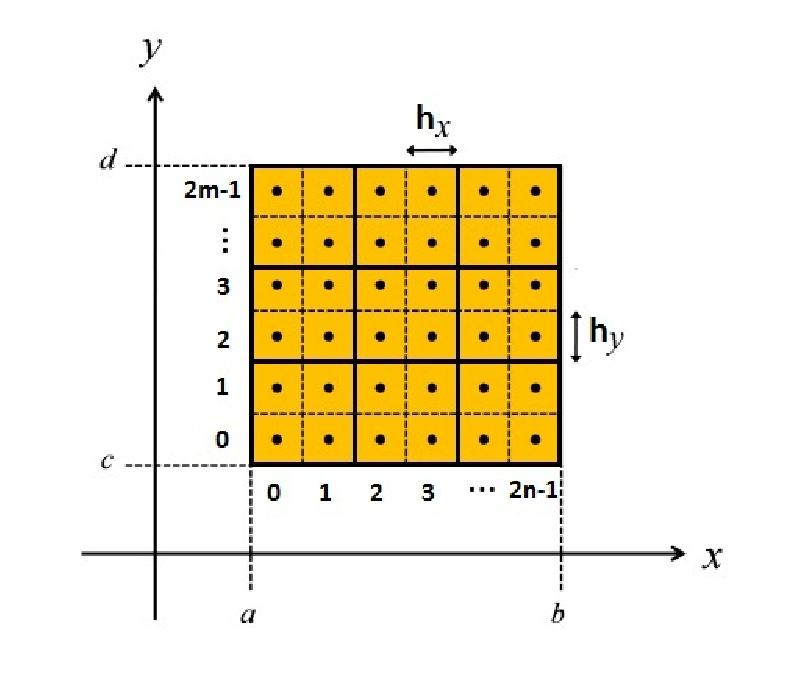
\includegraphics[scale=0.6]{R5.eps}
		\end{center}
	   \caption{Metoda Simpsona dla ca�ek podw�jnych po obszarze normalnym wzgl�dem dw�ch zmiennych - podzia� obszaru ca�kowania na podobszary }
\label{R5}
\end{figure}

Ka�dy z podobszar�w obszaru $\Omega$ jest ograniczonych pogrubion� kraw�dzi� i sk�ada si� zawsze z dok�adnie czterech mniejszych podpodobszar�w wyznaczanych przez dziewi�� w�z��w ($x_{2i},y_{2j}$) ( $i=0,1,\ldots, n$\,\,,\, \mbox{$j=0,1,\ldots, m$} ). Obj�to�� dowolnego z tych wi�kszych wyra�a wz�r:

\begin{equation}\label{ObjetoscPodobszaruSimpson2D}
\begin{array}{c}
S2V_{i,j}=\frac{h_xh_y}{9}\left[f(x_{2i},y_{2j})+4 f(x_{2i+1},y_{2j})+f(x_{2i+2},y_{2j})+\right.\\
4 f(x_{2i},y_{2j+1})+16 f(x_{2i+1},y_{2j+1})+4 f(x_{2i+2},y_{2j+1})+\\
\left.f(x_{2i},y_{2j+2})+4 f(x_{2i+1},y_{2j+1})+ f(x_{2i+2},y_{2j+2})\right]
\end{array}
\end{equation}\\       
Wsp�czynniki, kt�re pojawi�y si� w powy�szym zapisie przy warto�ciach funkcji $f(x,y)$  nie s� przypadkowe i tak intuicyjne jak dla \textit{wzoru Trapez�w}. Powsta�y one po przemno�eniu \textit{'okrojonej'} wersji wektor�w $A$ i $B$, kt�rych to u�ywali�my do wyprowadzenia macierzy (\ref{MacierzWspolczynnikowSimpson2}). %S� one postaci:

$$\qquad a= \left[
        \begin{array}{ccc}
         1 & 4 & 1 \\
         \end{array}
      \right],
      \qquad
 \,\,b= \left[
		\begin{array}{c}
         1 \\
         4\\
         1\\
         \end{array}       
     \right]. 
$$ 
W zwi�zku z tym ich iloczyn to:

\begin{equation}\label{MacierzWspolczynnikowSimpson2_objetosc1podobszaru}
a \times b = \left[
\begin{array}{ccc}
 		 1 & 4 & 1 \\
         4 & 16 & 4 \\
         1 & 4 & 1 \\
\end{array}
\right].
\end{equation}\\
 
Rozszerzaj�c zakres sumowania z jednego podobszaru na ca��  $\Omega$ nasz wz�r przyjmie ostatecznie bardziej czyteln� form�:
\begin{equation}\label{SumaObjetosciDlaCalegoObszaruSimpson2D}
\begin{array}{c}
I_{S2V}=I_{S2}\approx\frac{h_xh_y}{9}\sum\limits_{i=0}^{n-1}\sum\limits_{j=0}^{m-1}\left[f(x_{2i},y_{2j})+4 f(x_{2i+1},y_{2j})+f(x_{2i+2},y_{2j})+\right.\\
4 f(x_{2i},y_{2j+1})+16 f(x_{2i+1},y_{2j+1})+4 f(x_{2i+2},y_{2j+1})+\\
\left.f(x_{2i},y_{2j+2})+4 f(x_{2i+1},y_{2j+1})+ f(x_{2i+2},y_{2j+2})\right].
\end{array}
\end{equation}   
Zauwa�my, �e (\ref{SumaObjetosciDlaCalegoObszaruSimpson2D}) oraz (\ref{UogolnionyWzorSimpsona2_obszarNormalny}) s� r�wnowa�ne. Mo�na si� o tym przekona� rozpisuj�c (\ref{SumaObjetosciDlaCalegoObszaruSimpson2D}) ju� dla kilku pierwszych warto�ci $i$ oraz $j$.

Zaprezentowane dotychczas sposoby wyprowadzania \textit{uog�lnionego wzoru Simpsona} nie s� jedynymi nam znanymi. Poka�my, �e (zgodnie ze stwierdzeniem z pocz�tku rozdzia�u) to samo r�wnanie mo�emy otrzyma� poprzez ca�kowanie wielomianu \textit{Lagrange'a} $L_{2,2}(x,y)$. Ca�ka taka jest postaci:
\begin{equation}\label{WzorSimpsona2DZCalkiL22}
\int\limits_{x_0}^{x_2} \int\limits_{y_0}^{y_2} L_{2,2}(x,y) dydx=\int\limits_{x_0}^{x_2} \int\limits_{y_0}^{y_2} \sum\limits_{i=0}^2 \sum\limits_{j=0}^2 f(x_i,y_j) \left(\prod\limits_{s=0, s\neq i}^2 \frac{x-x_s}{x_i-x_s}\prod\limits_{r=0, r\neq j}^2 \frac{y-y_r}{y_j-y_r}\right)dydx
\end{equation}       
Przyjmuj�c nast�puj�ce warto�ci $x_0=0$, $x_1=h$, $x_2=2h$, $y_0=0$, $y_1=k$ oraz $y_2=2k$ mo�emy w (\ref{WzorSimpsona2DZCalkiL22}) wyszczeg�lni� dziewi�� ca�ek. Wyznaczenie ich spowoduje otrzymanie wsp�czynnik�w wyst�puj�cych przy warto�ciach funkcji $f(x_i,y_j)$ w kolejnych w�z�ach zgodnych z (\ref{MacierzWspolczynnikowSimpson2_objetosc1podobszaru}), tzn.:

\begin{small}
$$\int\limits_{x_0}^{x_2} \int\limits_{y_0}^{y_2} \frac{(x-x_1)(x-x_2)(y-y_1)(y-y_2)}{(x_0-x_1)(x_0-x_2)(y_0-y_1)(y_0-y_2)} dydx =\int\limits_{0}^{2h} \int\limits_{0}^{2k} \frac{(x-h)(x-2h)(y-k)(y-2k)}{(0-h)(0-2h)(0-k)(0-2k)} dydx = \frac{hk}{9}$$
$$\int\limits_{x_0}^{x_2} \int\limits_{y_0}^{y_2} \frac{(x-x_1)(x-x_2)(y-y_0)(y-y_2)}{(x_0-x_1)(x_0-x_2)(y_1-y_0)(y_1-y_2)} dydx =\int\limits_{0}^{2h} \int\limits_{0}^{2k} \frac{(x-h)(x-2h)(y-0)(y-2k)}{(0-h)(0-2h)(k-0)(k-2k)} dydx = \frac{4hk}{9}$$
$$\int\limits_{x_0}^{x_2} \int\limits_{y_0}^{y_2} \frac{(x-x_1)(x-x_2)(y-y_0)(y-y_1)}{(x_0-x_1)(x_0-x_2)(y_2-y_0)(y_2-y_1)} dydx =\int\limits_{0}^{2h} \int\limits_{0}^{2k} \frac{(x-h)(x-2h)(y-0)(y-k)}{(0-h)(0-2h)(2k-0)(2k-k)} dydx = \frac{hk}{9}$$

$$\int\limits_{x_0}^{x_2} \int\limits_{y_0}^{y_2} \frac{(x-x_0)(x-x_2)(y-y_1)(y-y_2)}{(x_1-x_0)(x_1-x_2)(y_0-y_1)(y_0-y_2)} dydx =\int\limits_{0}^{2h} \int\limits_{0}^{2k} \frac{(x-0)(x-2h)(y-k)(y-2k)}{(h-0)(h-2h)(0-k)(0-2k)} dydx = \frac{4hk}{9}$$
$$\int\limits_{x_0}^{x_2} \int\limits_{y_0}^{y_2} \frac{(x-x_0)(x-x_2)(y-y_0)(y-y_2)}{(x_1-x_0)(x_1-x_2)(y_1-y_0)(y_1-y_2)} dydx =\int\limits_{0}^{2h} \int\limits_{0}^{2k} \frac{(x-0)(x-2h)(y-0)(y-2k)}{(h-0)(h-2h)(k-0)(k-2k)} dydx = \frac{16hk}{9}$$
$$\int\limits_{x_0}^{x_2} \int\limits_{y_0}^{y_2} \frac{(x-x_0)(x-x_2)(y-y_0)(y-y_1)}{(x_1-x_0)(x_1-x_2)(y_2-y_0)(y_2-y_1)} dydx =\int\limits_{0}^{2h} \int\limits_{0}^{2k} \frac{(x-0)(x-2h)(y-0)(y-k)}{(h-0)(h-2h)(2k-0)(2k-k)} dydx = \frac{4hk}{9}$$

$$\int\limits_{x_0}^{x_2} \int\limits_{y_0}^{y_2} \frac{(x-x_0)(x-x_1)(y-y_1)(y-y_2)}{(x_2-x_0)(x_2-x_1)(y_0-y_1)(y_0-y_2)} dydx =\int\limits_{0}^{2h} \int\limits_{0}^{2k} \frac{(x-0)(x-h)(y-k)(y-2k)}{(2h-0)(2h-h)(0-k)(0-2k)} dydx = \frac{hk}{9}$$
$$\int\limits_{x_0}^{x_2} \int\limits_{y_0}^{y_2} \frac{(x-x_0)(x-x_1)(y-y_0)(y-y_2)}{(x_2-x_0)(x_2-x_1)(y_1-y_0)(y_1-y_2)} dydx =\int\limits_{0}^{2h} \int\limits_{0}^{2k} \frac{(x-0)(x-h)(y-0)(y-2k)}{(2h-0)(2h-h)(k-0)(k-2k)} dydx = \frac{4hk}{9}$$
$$\int\limits_{x_0}^{x_2} \int\limits_{y_0}^{y_2} \frac{(x-x_0)(x-x_1)(y-y_0)(y-y_1)}{(x_2-x_0)(x_2-x_1)(y_2-y_0)(y_2-y_1)} dydx =\int\limits_{0}^{2h} \int\limits_{0}^{2k} \frac{(x-0)(x-h)(y-0)(y-k)}{(2h-0)(2h-h)(2k-0)(2k-k)} dydx = \frac{hk}{9}$$

\end{small}\hfill\\
Tak jak wspomnieli�my tu� przed przeprowadzeniem oblicze�, powy�ej wyznaczone wsp�czynniki tworz� macierz (\ref{MacierzWspolczynnikowSimpson2_objetosc1podobszaru}). Wyja�niaj�c - ka�de kolejne trzy warto�ci pocz�wszy od pierwszej, czwartej i si�dmej tworz� jeden osobny jej wiersz. Obliczenia te s� bardzo pracoch�onne, zosta�y wi�c zaprezentowane tylko w celach pogl�dowych.  

Wykorzystuj�c (\ref{UogolnionyWzorSimpsona2_obszarNormalny}) lub sam� macierz (\ref{MacierzWspolczynnikowSimpson2}) wyznaczmy przybli�on� warto�� pewnej ca�ki, mianowicie:

\begin{ex}(Wyznaczanie warto�ci ca�ki podw�jnej \textit{wzorem Simpsona})\\\hfill
\textit{Obliczymy  $\int\limits_{0}^{\frac{1}{2}}\int\limits_{\frac{1}{2}}^1 \frac{x+y}{x^2+y^2}dydx$ wykorzystuj�c uog�lniony wz�r Simpsona dla ca�ek podw�jnych po obszarach normalnych. Dla rozpatrywanego przypadku przyjmijmy, �e przedzia� ca�kowania zar�wno dla zmiennej $x$ jak i $y$ zostanie podzielony na dwa podw�jne podprzedzia�y wyznaczone przez r�wno odleg�e w�z�y. }\\

\hspace{-1cm}Z powy�szego opisu wynika, �e b�dziemy potrzebowa� $n=5$ wsp�rz�dnych $x$ oraz $m=5$ wsp�rz�dnych $y$.
Podzia� przedzia��w ca�kowania przyjmuj�c, �e $h_x=\frac{\frac{4}{8}-0}{4}=\frac{4}{32}=\frac{1}{8}$ oraz $h_y=\frac{1-\frac{4}{8}}{4}=\frac{4}{32}=\frac{1}{8}$ prezentuje si� nast�puj�co:
$$x_0=0,\, x_1=\frac{1}{8},\, x_2=\frac{2}{8},\, x_3=\frac{3}{8},\, x_4=\frac{4}{8}$$
$$y_0=\frac{4}{8},\, y_1=\frac{5}{8},\, y_2=\frac{6}{8},\, y_3=\frac{7}{8},\, y_4=1.$$ 

Do oblicze� wykorzystamy wz�r rozpisany na podstawie (\ref{MacierzWspolczynnikowSimpson2}):
$$\int\limits_{0}^{\frac{1}{2}}\int\limits_{\frac{1}{2}}^1 \frac{x+y}{x^2+y^2}dydx\approx
\frac{h_xh_y}{9} \left(f(x_0,y_0)+4f(x_1,y_0)+2f(x_2,y_0)+4f(x_3,y_0)+f(x_4,y_0)+\right.$$
$$4f(x_0,y_1)+16f(x_1,y_1)+8f(x_2,y_1)+16f(x_3,y_1)+4f(x_4,y_1)+$$
$$ 2f(x_0,y_2)+8f(x_1,y_2)+4f(x_2,y_2)+8f(x_3,y_2)+2(x_4,y_2)+$$
$$4f(x_0,y_3)+16f(x_1,y_3)+8f(x_2,y_3)+16f(x_3,y_3)+4f(x_4,y_3)+$$
$$\left.f(x_0,y_4)+4f(x_1,y_4)+2f(x_2,y_4)+4f(x_3,y_4)+f(x_4,y_4)\right)=$$
$$=\frac{\frac{1}{8}\frac{1}{8}}{9}\left( \frac{\frac{4}{8}}{\left(\frac{4}{8}\right)^2} + 4\cdot \frac{\frac{5}{8}}{\left(\frac{1}{8}\right)^2+\left(\frac{4}{8}\right)^2} + 2 \cdot \frac{\frac{6}{8}}{\left(\frac{2}{8}\right)^2+\left(\frac{4}{8}\right)^2} + 4 \cdot \frac{\frac{7}{8}}{\left(\frac{3}{8}\right)^2+\left(\frac{4}{8}\right)^2} +\frac{1}{\left(\frac{4}{8}\right)^2+\left(\frac{4}{8}\right)^2} +  \right.$$
$$4\cdot\frac{ \frac{5}{8}}{\left(\frac{5}{8}\right)^2} + 16\cdot \frac{\frac{6}{8}}{\left(\frac{1}{8}\right)^2+\left(\frac{5}{8}\right)^2} + 8 \cdot \frac{\frac{7}{8}}{\left(\frac{2}{8}\right)^2+\left(\frac{5}{8}\right)^2} + 16 \cdot \frac{1}{\left(\frac{3}{8}\right)^2+\left(\frac{5}{8}\right)^2} + 4\cdot\frac{\frac{9}{8}}{\left(\frac{4}{8}\right)^2+\left(\frac{5}{8}\right)^2} +$$
$$2\cdot\frac{ \frac{6}{8}}{\left(\frac{6}{8}\right)^2} + 8\cdot \frac{\frac{7}{8}}{\left(\frac{1}{8}\right)^2+\left(\frac{6}{8}\right)^2} + 4 \cdot \frac{1}{\left(\frac{2}{8}\right)^2+\left(\frac{6}{8}\right)^2} + 8 \cdot \frac{\frac{9}{8}}{\left(\frac{3}{8}\right)^2+\left(\frac{6}{8}\right)^2} + 2\cdot\frac{\frac{10}{8}}{\left(\frac{4}{8}\right)^2+\left(\frac{6}{8}\right)^2} +$$
$$4\cdot\frac{ \frac{7}{8}}{\left(\frac{7}{8}\right)^2} + 16\cdot \frac{1}{\left(\frac{1}{8}\right)^2+\left(\frac{7}{8}\right)^2} + 8 \cdot \frac{\frac{9}{8}}{\left(\frac{2}{8}\right)^2+\left(\frac{7}{8}\right)^2} + 16 \cdot \frac{\frac{10}{8}}{\left(\frac{3}{8}\right)^2+\left(\frac{7}{8}\right)^2} + 4\cdot\frac{\frac{11}{8}}{\left(\frac{4}{8}\right)^2+\left(\frac{7}{8}\right)^2} +$$
$$\left.1 + 4\cdot \frac{\frac{9}{8}}{\left(\frac{1}{8}\right)^2+\left(1\right)^2} + 2 \cdot \frac{\frac{10}{8}}{\left(\frac{2}{8}\right)^2+\left(1\right)^2} + 4 \cdot \frac{\frac{11}{8}}{\left(\frac{3}{8}\right)^2+\left(1\right)^2} +\frac{\frac{12}{8}}{\left(\frac{4}{8}\right)^2+\left(1\right)^2} \right) \approx$$
$$\approx\frac{1}{576}\cdot(27,17176470588235 + 88,52877470325647 + 37,05169785169785 + $$
$$+ 63,40370323235645 + 13,80562821545899)\approx 0,399238834563632$$

W zaokr�gleniu warto�� dok�adna rozwi�zywanej ca�ki, otrzymana przy wykorzystaniu kalkulatora to: $\int\limits_{0}^{\frac{1}{2}}\int\limits_{\frac{1}{2}}^1 \frac{x+y}{x^2+y^2}dydx \approx 0.399181467986060$

Analizuj�c wielko�� b��du wzgl�dnego (\textbf{BW}), kt�rym jest obci��ony wynik, zauwa�amy �e nie jest znacz�cy i wynosi jedynie $0,014\%$. Wynika to z poni�szych rachunk�w: 
\begin{center}
$BW = \frac{|0,399181467986 - 0,399238834563632|}{0,399181467986} * 100\% \approx 0,01437\%\approx 0,014\% $ \\
\end{center}
%W tym momencie uwidacznia si� zdecydowanie wi�ksza dok�adno�� \textit{uog�lnionego wzoru Simpsona} w zestawieniu go z \textit{uog�lnionym wzorem Trapez�w}. 
Dla \textit{wzoru trapez�w }wielko�� BW (dla takiej samej ca�ki) przy wykonanych dw�ch podzia�ach przedzia�u ca�kowania oscylowa�a w granicach $0,2\%$, wi�c by�a ona niemal 15 krotnie wi�ksza!
\end{ex}
Algorytm \textit{Simpsona} (\ref{SumaObjetosciDlaCalegoObszaruSimpson2D}) pomimo tego, �e na pierwszy rzut oka wydaje si� by� skuteczniejszy ni�  wspomniany \textit{wz�r Trapez�w} (\ref{RownoscUogWzoruTrapezow2IWzoruZObjetosciami}), to jest r�wnie� du�o bardziej skomplikowany je�eli chodzi o z�o�ono�� rachunk�w jakie nale�y wykona�. Ka�de zwi�kszenie liczby w�z��w powoduje bardzo szybki rozrost ilo�ci warto�ci funkcji do wyznaczenia. W zwi�zku z tym, by kontynuowa� rozwa�ania zaprezentujmy stworzon� procedur� automatyzuj�c� obliczanie warto�ci ca�ek podw�jnych po obszarach normalnych \textit{uog�lnionym wzorem Simpsona}.
\begin{proc}(Wyznaczanie przybli�onych warto�ci ca�ek podw�jnych po obszarach normalnych przy u�yciu uog�lnionego wzoru Simpsona)\label{MAPLE_Simpson2ObszarNormalnyWartoscCalki}
\begin{small}
\begin{verbatim}
> Simpson2 := proc(a, b, c, d, N, M) 
local h, k, i, j, n, m, p, q, x, y, z, S2, WynikS2; 
if ((((ceil(N)>N) or (floor(N)<N)) or (mod(N,2) = 1 and N>0) or N <= 0)
or (((ceil(M)>M) or (floor(M)<M)) or (mod(M,2) = 1 and M>0) or M <= 0)) 
then 
ERROR('Ostatnie dwa parametry musza byc liczba naturalna postaci \2k') 

else 
n := (1/2)*N; 
m := (1/2)*M; 
h := (b-a)/N; 
k := (d-c)/M; 

for i from 0 to N 
do x := i -> a+i*h od; 

for j from 0 to M 
do y := j -> c+j*k od; 

for i from 0 to N 
do for j from 0 to M 
do z :=(i,j) -> f(x(i),y(j)) od
od; 

S2 := (1/9)*h*k*(sum(sum(z(2*p,2*q)+4*z(2*p+1,2*q)+z(2*p+2,2*q)
+4*z(2*p,2*q+1)+16*z(2*p+1,2*q+1)+4*z(2*p+2,2*q+1)
+z(2*p,2*q+2)+4*z(2*p+1,2*q+2)+z(2*p+2,2*q+2)
, p = 0 .. n-1), q = 0 .. m-1)); 

WynikS2 := evalf(S2) fi; 
end;
\end{verbatim}
\end{small}
\end{proc}  

Pierwsza linia powy�szego kodu jest deklaracj� nazwy procedury oraz jej parametr�w wej�ciowych, przy czym:\\
a, b -  dolna i g�rna granica ca�kowania wzgl�dem zmiennej $x$,\\
c, d -  dolna i g�rna granica ca�kowania wzgl�dem zmiennej $y$,\\
N - liczba podpodprzedzia��w na jakie zostanie podzielony ca�y przedzia� ca�kowania $[a,b]$,\\
M - liczba podpodprzedzia��w na jakie zostanie podzielony ca�y przedzia� ca�kowania $[c,d]$.\\
Kolejno wymienione s� wszystkie zmienne lokalne, jakie b�d� wykorzystane w obliczeniach wykonywanych wewn�trz algorytmu. Pojawiaj�ca si� nast�pnie instrukcja warunkowa \textit{if-else} decyduje o tym, czy parametry wywo�ania zosta�y podane prawid�owo. Je�eli $N$ lub $M$ nie jest liczb� naturaln� parzyst� to zwracany jest stosowny komunikat o b��dzie. W przeciwnym przypadku rozpoczyna si� wykonanie w�a�ciwej cz�ci algorytmu, w sk�ad kt�rego wchodzi okre�lenie ilo�ci podprzedzia��w $n$, $m$ (ka�dy podprzedzia� z�o�ony jest z dw�ch podpodprzedzia��w) na kt�re podzielono przedzia�y ca�kowania po zmiennej $x$ i $y$. Dalej na podstawie (\ref{WezlyNaObszarzeProstokatnymSimpson2}) wyznaczane s� wielko�ci krok�w $h$ (dla $x$) i $k$ (dla $y$) pomi�dzy kolejnymi w�z�ami definiuj�cymi kra�ce owych podpodprzedzia��w. Pozyskane dane zostaj� natychmiast wykorzystywane przez p�tle \textit{for} do obliczenia wsp�rz�dnych w�z��w $x_i$ oraz $y_j$. Blok z dwoma zagnie�d�onymi p�tlami \textit{for} s�u�y wyliczaniu warto�ci funkcji $z(i,j)=f(x_i,y_j)$ w okre�lonych (w poprzednich dw�ch krokach) punktach w�z�owych. Przedostatni krok jest implementacj� wzoru (\ref{SumaObjetosciDlaCalegoObszaruSimpson2D}), co czyni go kluczowym dla ca�ego algorytmu. Ostatecznie wynik procedury jest zwracany w uproszczonej i czytelnej postaci jako warto�� \textit{WynikS2}.

Wiedz�c ju� na jakiej zasadzie dzia�a procedura \textit{Simpson2} - u�yjmy jej do przeprowadzenia bada� nad dok�adno�ci� pozyskanych dzi�ki niej przybli�onych wynik�w ca�kowania. Rezultaty por�wnamy z tymi, otrzymanymi przez procedur� \ref{MAPLE_Trapez2ObszarNormalnyWartoscCalki} (\textit{Trapez2}). Przeliczmy zatem nast�puj�ce ca�ki: 
\begin{itemize}
\item[a)] $\int\limits_0^\frac{1}{2}\int\limits_\frac{1}{2}^1 \frac{x+y}{x^2+y^2} dydx$
\item[b)] $\int\limits_0^1\int\limits_1^2 e^\frac{x^2}{y^3} dydx$
\end{itemize}
Tak jak w  podrozdziale poprzednim wyniki przedstawimy w formie tabel. Niech $N$ oznacza liczb� podpodprzedzia��w na kt�re podzielono przedzia� ca�kowania po zmiennej $x$, $M$ po zmiennej $y$, $W_{Simpson2}$ to wynik \textit{Simpson2} dla rosn�cych warto�ci $N$ i $M$. Niech \textit{$BBS2_{N,M}$} b�dzie b��dem bezwzgl�dnym przybli�enia warto�ci ca�ki podw�jnej procedur� \textit{Simpson2} dla pewnych parametr�w $N$ i $M$. Dodatkowo \textit{$BWS2_{N,M}$} to wielko�� b��du wzgl�dnego jakim jest obci��ony ten sam wynik wykonania \textit{Simpson2}, co w przypadku wyliczania \textit{$BBS2_{N,M}$}.\\

Warto�� ca�ki z przyk�adu a) jest w zaokr�gleniu r�wna $0,399181467986$, wi�c:
\begin{table}[h!]
\centering
 \begin{tabular}{|c|c|c|c|c|} 
 \hline
 $\mathbf{N}$ &$\mathbf{M}$ & $\mathbf{W_{Simpson2}}$ & $\mathbf{BBS2_{N,M}}$ &$\mathbf{BWS2_{N,M}}$ \\ %[0.5ex] 
 \hline \hline
 2&4 &0.399628737181  &0.000447269195  &0.112046583038 \%  \\  
  \hline 
 4&4 &0.399238834564  &0.000057366578  &0.014371052416 \% \\ 
  \hline
 8&4 &0.399209961856  &0.000028493870     &0.007138074356 \% \\ 
  \hline 
 16&20 &0.399181624022  &0.000000156036   &0.000039088989 \% \\ 
  \hline 
 30&20 &0.399181522060  &0.000000054074   &0.000013546220 \% \\ 
  \hline 
 60&20 &0.399181513672  &0.000000045686   &0.000011444920 \% \\ 
  \hline 
 90&50 &0.399181469254  &0.000000001268   &0.000000317650 \% \\ 
  \hline
 120&50 &0.399181469179  &0.000000001193  &0.000000298862 \% \\  
  \hline 
 150&50 &0.399181469158  &0.000000000117  &0.000000293600 \% \\ 
  \hline 
 180&100 &0.399181468065  &0.000000000079 &0.000000019790 \% \\ 
  \hline
 200&100 &0.399181468063  &0.000000000077 &0.000000019289 \% \\ 
  \hline 
 230&100 &0.399181468061  &0.000000000075 &0.000000018788 \% \\  
  \hline 
 260&200 &0.399181467992  &0.0000000000006 &0.000000001503 \% \\ 
   \hline 
 300&200 &0.399181467991  &0.0000000000005 &0.000000001253 \% \\ 
  \hline               
 400&200 &0.399181467991  &0.0000000000005  &0.000000001253  \%  \\%[0.5ex] 
 \hline 
 \end{tabular}\\ \hfill
 \caption{Pomiary dok�adno�ci przybli�ania warto�ci ca�ki a) \textit{uog�lnionym wzorem Simpsona}}
 \label{WynikiZProcedurySimpson2a}
\end{table}
\\ 

Ca�ka z podpunktu b) wynosi dok�adnie $1.14782135872$ , zatem:. 
\begin{table}[h!]
\centering
 \begin{tabular}{|c|c|c|c|c|} 
 \hline
 $\mathbf{N}$ &$\mathbf{M}$ & $\mathbf{W_{Simpson2}}$ & $\mathbf{BBS2_{N,M}}$ &$\mathbf{BWS2_{N,M}}$ \\ %[0.5ex] 
  \hline \hline
 2&4 &1.15087844676    &0.00305708804   &0.266338312733 \%  \\  
  \hline 
 4&4 &1.14909546116    &0.00127410244   &0.111001806189 \% \\ 
  \hline
 8&4 &1.14895802395    &0.00113666523   &0.099028060539 \% \\ 
  \hline 
 16&20 &1.14782496457  &0.00000360585   &0.000314147317 \% \\ 
  \hline 
 30&20 &1.14782444884  &0.00000309012   &0.000269216109 \% \\ 
  \hline 
 60&20 &1.14782440610  &0.00000304738   &0.000265492533 \% \\ 
  \hline 
 90&50 &1.14782144016  &0.00000008144   &0.000007095181 \% \\ 
  \hline
 120&50 &1.14782143971 &0.00000008099   &0.000007055976 \% \\ 
  \hline 
 150&50 &1.14782143962  &0.00000008090  &0.000007048135 \% \\ 
  \hline 
 180&100 &1.14782136425  &0.00000000554  &0.000000481782 \% \\ 
  \hline
 200&100 &1.14782136416 &0.00000000544  &0.000000473941 \% \\ 
  \hline 
 230&100 &1.14782136423  &0.00000000551  &0.000000480039 \% \\  
  \hline 
 260&200 &1.14782135945  &0.00000000126  &0.000000063598 \% \\ 
   \hline 
 300&200 &1.14782135952  &0.00000000081  &0.000000070568 \% \\ 
  \hline               
 400&200 &1.14782135935  &0.00000000063 & 0.000000054886 \%  \\%[0.5ex] 
 \hline 
 \end{tabular}\\ \hfill
 \caption{Pomiary dok�adno�ci przybli�ania warto�ci ca�ki b) \textit{uog�lnionym wzorem Simpsona}}
 \label{WynikiZProcedurySimpson2b}
\end{table}


Dokonuj�c przegl�du i analizy wynik�w z Tablicy \ref{WynikiZProcedurySimpson2a} i Tablicy \ref{WynikiZProcedurySimpson2b} pierwsze co powinno rzuci� si� nam w oczy to wyj�tkowa dok�adno�� otrzymanych warto�ci. Wielko�� b��du bezwzgl�dnego ju� dla pierwszego wywo�ania procedury w obydwu przyk�adach nie przekroczy�a $0.0031$, jest to bardzo dobry rezultat. Dodatkowo po ka�dym zwi�kszeniu parametr�w $N$ lub $M$ widoczna jest stanowcza tendencja spadkowa \textbf{$BBS2_{N,M}$} jak i \textbf{$BWS2_{N,M}$}. Dla ko�cowych pomiar�w mo�na powiedzie�, �e wynik jest niemal nie obci��ony b��dem przybli�enia, poniewa� jego wielko�� jest bliska $0$ dla obydwu przyk�ad�w. Interesuj�ce jest to, �e pomi�dzy b��dami, kt�rymi obci��one s� wyniki otrzymane \textit{uog�lnionym wzorem trapez�w} a \textit{uog�lnionym wzorem Simpsona} jest �rednio dwa rz�dy wielko�ci r�nicy (na korzy�� wzoru \textit{Simpsona}). Fakt ten sprawia, �e mo�e on zosta� uznany za dok�adniejszy i zarazem bardziej efektywny.    









%\section{Wz�r 'prostok�t�w'}

\chapter{Kwadratury Newtona-Cotesa dla ca�ek podw�jnych w obszarach normalnych}
\section{Wz�r trapez�w dla obszaru normalnego wed�ug osi Ox}
\section{Wz�r Simpsona dla obszaru normalnego wed�ug osi Ox}
\section{Wz�r trapez�w dla obszaru normalnego wed�ug osi Oy}
\section{Wz�r Simpsona dla obszaru normalnego wed�ug osi Oy}



   
   
   
   
   
\chapter*{Podsumowanie}
Celem pracy by�o wyprowadzenie wybranych \textit{dwuwymiarowych kwadratur Newtona-Cotesa} (tzn. \textit{uog�lniony wz�r trapez�w} i \textit{uog�lniony wz�r Simpsona}) dla ca�ek podw�jnych w prostok�cie oraz w obszarze normalnym wzgl�dem osi $Ox$ czy te� osi $Oy$. W ramach wprowadzenia do tematyki w rozdziale drugim zaprezentowano tak�e te same kwadratury dla oznaczonych ca�ek pojedynczych. Ponadto skupili�my si� mi�dzy innymi na badaniu dok�adno�ci z jak� owe wzory  przybli�aj� w�a�ciwe warto�ci oznaczonych ca�ek pojedynczych i podw�jnych. Wszystkie z zaplanowanych we wst�pnie wzor�w  z sukcesem uda�o si� wyprowadzi�. Dla ka�dego przypadku powsta� stosowny podrozdzia� pracy w kt�rym zamieszczano kompletne przekszta�cenia prowadz�ce do otrzymania wzor�w, niejednokrotnie rozwi�zania przyk�adowych zada� jak r�wnie� i procedury j�zyka \textit{Maple} wspomagaj�ce wykonywanie pomiar�w wykorzystanych do bada�. Analiza otrzymanych wynik�w pokazuje, �e dla przypadku ca�ek podw�jnych \textit{metoda Simpsona} jest zawsze dok�adniejsza od \textit{metody trapez�w}.  


Kierunkiem dalszego rozwoju pracy mo�e by� np. wyznaczenie wzor�w opisanych prezentowanych kwadratur zar�wno dla ca�ek potr�jnych jak te� i ca�ek podw�jnych w obszarach, kt�re nie s� normalne wzgl�dem �adnej z osi. Z nowo wyprowadzonymi wzorami mog�oby tak�e wi�za� si� przeprowadzenie bada� nad ich dok�adno�ci� przybli�ania wyniku.          
\addcontentsline{toc}{chapter}{Podsumowanie}





%================Bibliografia===============
\bibliographystyle{unsrt}
\begin{thebibliography}{99}

\bibitem{klucz1} Olszowski B.,\,\,\textit{Wybrane metody numeryczne : podr�cznik dla student�w wy�szych szk� technicznych}, Wydawnictwo Politechniki Krakowskiej, Krak�w 2007, s. 27-37

\bibitem{klucz2} Kosma Z.,\,\,\textit{Metody numeryczne dla zastosowa� in�ynierskich}, Wydawnictwo Politechniki Radomskiej, Radom 2007, s. 155-160

\bibitem{klucz3} 

\bibitem{klucz4} 

\end{thebibliography}

\addcontentsline{toc}{chapter}{Bibliografia} % bibliografia dodana do spisu tresci jako rozdzial




%=================Spis procedur============
\newpage
\renewcommand{\listoftables}{\Large\textbf{\flushleft{Spis procedur w j�zyku Maple}}}
\listoftables


\addcontentsline{toc}{chapter}{Spis procedur w j�zyku Maple}



%\listoffigures
%\addcontentsline{toc}{chapter}{Spis rysunk�w}

\end{document}
